\documentclass[10pt, c, xcolor=x11names]{beamer}\usepackage[]{graphicx}\usepackage[]{color}
%% maxwidth is the original width if it is less than linewidth
%% otherwise use linewidth (to make sure the graphics do not exceed the margin)
\makeatletter
\def\maxwidth{ %
  \ifdim\Gin@nat@width>\linewidth
    \linewidth
  \else
    \Gin@nat@width
  \fi
}
\makeatother

\definecolor{fgcolor}{rgb}{0.345, 0.345, 0.345}
\newcommand{\hlnum}[1]{\textcolor[rgb]{0.686,0.059,0.569}{#1}}%
\newcommand{\hlstr}[1]{\textcolor[rgb]{0.192,0.494,0.8}{#1}}%
\newcommand{\hlcom}[1]{\textcolor[rgb]{0.678,0.584,0.686}{\textit{#1}}}%
\newcommand{\hlopt}[1]{\textcolor[rgb]{0,0,0}{#1}}%
\newcommand{\hlstd}[1]{\textcolor[rgb]{0.345,0.345,0.345}{#1}}%
\newcommand{\hlkwa}[1]{\textcolor[rgb]{0.161,0.373,0.58}{\textbf{#1}}}%
\newcommand{\hlkwb}[1]{\textcolor[rgb]{0.69,0.353,0.396}{#1}}%
\newcommand{\hlkwc}[1]{\textcolor[rgb]{0.333,0.667,0.333}{#1}}%
\newcommand{\hlkwd}[1]{\textcolor[rgb]{0.737,0.353,0.396}{\textbf{#1}}}%
\let\hlipl\hlkwb

\usepackage{framed}
\makeatletter
\newenvironment{kframe}{%
 \def\at@end@of@kframe{}%
 \ifinner\ifhmode%
  \def\at@end@of@kframe{\end{minipage}}%
  \begin{minipage}{\columnwidth}%
 \fi\fi%
 \def\FrameCommand##1{\hskip\@totalleftmargin \hskip-\fboxsep
 \colorbox{shadecolor}{##1}\hskip-\fboxsep
     % There is no \\@totalrightmargin, so:
     \hskip-\linewidth \hskip-\@totalleftmargin \hskip\columnwidth}%
 \MakeFramed {\advance\hsize-\width
   \@totalleftmargin\z@ \linewidth\hsize
   \@setminipage}}%
 {\par\unskip\endMakeFramed%
 \at@end@of@kframe}
\makeatother

\definecolor{shadecolor}{rgb}{.97, .97, .97}
\definecolor{messagecolor}{rgb}{0, 0, 0}
\definecolor{warningcolor}{rgb}{1, 0, 1}
\definecolor{errorcolor}{rgb}{1, 0, 0}
\newenvironment{knitrout}{}{} % an empty environment to be redefined in TeX

\usepackage{alltt}

\def\currentChapter{Variable Selection and Regularization}


% THEME BEAMER
\usepackage{../themeJC2BIM}

\graphicspath{{figures/},{../common_figs/}}
\usepackage{tikz}
\usetikzlibrary{calc,shapes,backgrounds,arrows,automata,shadows,positioning}
\tikzstyle{every state}=[fill=red,draw=none,scale=0.7,font=\small,text=white]
\tikzstyle{every edge}=[-,shorten >=1pt,auto,thin,draw]
\tikzstyle{alertstate}=[fill=bleu]
\definecolor{genecolor}{RGB}{94,135,173}

\def\currentDate{Fréjus, 4--8 June 2018}
\def\currentInstitute{Julien Chiquet}
\def\currentCourse{(JC)2BIM 2018 Research School}

\title{\currentCourse}

\subtitle{\huge\currentChapter\normalsize}

\institute{\currentInstitute}

\date{\currentDate}



\AtBeginSection{
  \begin{frame}<beamer>
    \frametitle{Outline}
    \framesubtitle{\insertpart}
    \tableofcontents[currentsection,currentsubsection, subsectionstyle=show/shaded/hide]  
  \end{frame}
}

\AtBeginSubsection{
  \begin{frame}<beamer>
    \frametitle{Outline}
    \framesubtitle{\insertpart}
    \tableofcontents[currentsection,currentsubsection, subsectionstyle=show/shaded/hide]  
  \end{frame}
}

\AtBeginSubsubsection{
  \begin{frame}<beamer>
    \frametitle{Outline}
    \framesubtitle{\insertpart}
    \tableofcontents[currentsection,currentsubsection, subsectionstyle=show/shaded/hide]  
  \end{frame}
}

\newcommand{\dotitlepage}{%
  \begin{frame}
    \titlepage
    \vfill
    \begin{center}
        \scriptsize\url{http://github/jchiquet/JC2BIM}
    \end{center}
    \vfill
    
\includegraphics[width=1.5cm]{logo_cnrs}\hfill
    
\includegraphics[width=2.5cm]{logo_inra}
  \end{frame}
  %
}

\newcommand{\dotoc}{%
  \begin{frame}
    \frametitle{Outline}
    \tableofcontents[currentsection,
    sectionstyle=show/show,
    subsectionstyle=hide]
  \end{frame}
  %
}



\IfFileExists{upquote.sty}{\usepackage{upquote}}{}
\begin{document}

\dotitlepage

\dotoc

\section{Motivations}


\subsection{Assessing the quality of a regression model}

\begin{frame}
  \frametitle{Statistical Learning}

  \begin{block}{Canonical scenario}
    \begin{enumerate}
    \item an \alert{outcome} measurement (or \emph{response}, \emph{output})
      \begin{itemize}
      \item  either   quantitative  (expression  level,   tumor  size,
        survival time, etc.)
      \item or categorical (presence/absence of a gene or of a disease, etc.)
      \end{itemize}
    \item a set of  \alert{features} (or \emph{predictors}, \emph{inputs})
      \begin{itemize}
      \item clinical measurements (expression level, tumor size)
      \item age, smoking or not, height, SNPs, etc.
      \end{itemize}
    \end{enumerate}
  \end{block}

  \vfill

  \begin{block}{Learning problem} Given a training set of data (observed
    inputs and outputs), we aim to
    \begin{enumerate}
    \item suggest a model,
    \item learn this model on the training set,
    \item test this model on new outcomes/features.
    \end{enumerate}
  \end{block}

  \vfill

  $\rightsquigarrow$   \alert{A  ``good''   model  should   accurately
    predict new outcomes.}
\end{frame}

\begin{frame}
  \frametitle{Notations}

  Let
  \begin{itemize}
  \item $Y$ be the output random variable,
  \item  $X  =  (X_1,  \dots,  X_p)$  be  the  input  random
    variables, where $X_j$ is the $j$ predictor.
  \end{itemize}

  \vfill

  \begin{block}{The data}
    Given a sample $\{(y_i, x_i), i=1,\dots,n\}$ of i.id. realizations
    of $(Y,X)$, denote
    \begin{itemize}
    \item $\mathcal{D} = \{i:(y_i, x_i) \in \text{ training set}\}$,
    \item $\mathcal{T} = \{i:(y_i, x_i) \in \text{ test set}\}$,
    \item   $\mathbf{y}   =   (y_i)_{i\in\mathcal{D}}$,  the
      \emph{response} vector in $\mathbb{R}^{|\mathcal{D}|}$,
    \item $\mathbf{x}_j =  (x_{ij})_{i\in\mathcal{D}}^\intercal)$ the vector
      of data for the $j$th predictor in $\mathbb{R}^{|\mathcal{D}|}$,
    \item $\mathbf{X}$ the $n\times p$  data (or design) matrix on the
      training set whose $j$th row is $\mathbf{x}_j$,
    \item $(\by_\mathcal{T},\bX_\mathcal{T})$ are the test data.
    \end{itemize}
  \end{block}
\end{frame}

\begin{frame}
  \frametitle{Regression models}

  We seek a function $f$ that predicts $Y$ through $X$.

  \begin{proposition} The  model $f(X)=\E[Y|X]$ minimizes  the squared
    error loss, that is,
    \begin{equation*}
      f(X)   =    \argmin_{\varphi}   \err(\varphi(X)),   \quad
      \text{with } \err(\varphi(X)) = \mathbb{E}[(Y - \varphi(X))^2].
    \end{equation*}
    $\rightsquigarrow$ The best prediction of $Y$ at any point $X = x$
    is the conditional mean, when  best is measured by average squared
    error.
  \end{proposition}

  \vfill

  This leads to the regression model
    \begin{equation*}
      Y = f(X) + \varepsilon,
    \end{equation*}
    where
    \begin{itemize}
    \item     $\varepsilon$     is     an    additive     error     with
      $\E[\varepsilon]=\mathbf{0}$, $\var[\varepsilon]=\sigma^2$,
    \item $f(x) = \E[Y | X = x]$ is the \emph{regression} function.
    \end{itemize}

\end{frame}

\begin{frame}
  \frametitle{Learning strategy}

  \begin{block}{Problem}
    $\prob(Y|X)$  and  $\prob(X)$   are  unknown  thus  $\E(Y|X),  \err(f(X))$
  unreachable: one should \alert{estimate} this.
  \end{block}

  \vfill

  \begin{block}{Strategy}
    \begin{enumerate}
    \item  Fix a family $\mathcal{F}$ of models\\
        \onslide<2>{\textit{For the linear model, $\mathcal{F} = \set{X^T\bbeta, \bbeta\in\Rset^p}$.}}
      \bigskip
    \item Fit a model $\hat{f}\in\mathcal{F}$ on the training set $\mathcal{D}$\\ 
      \onslide<2>{\textit{With the least square, compute $\hatbbetaols$ and $\hat f = \hat Y = \bX \hatbbetaols$}}\bigskip
    \item Estimate the prediction error with the test set $\mathcal{T}$.
       \begin{equation*}
         \onslide<2>{\text{For instance, }\hat{\err}(\bX_{\mathcal{T}}\hatbbetaols) = \frac{1}{n} \left\|
         \by_{\mathcal{T}}- \bX_{\mathcal{T}} \hatbbetaols_{\mathcal{D}}\right\|^2.}
       \end{equation*}
    \end{enumerate}
  \end{block}
\end{frame}

\begin{frame}
  \frametitle{Bias/variance tradeoff}

  At an input point $X=x$,
  \begin{overlayarea}{\textwidth}{\textheight}
    \begin{equation*}
      \err(\hat{f}(x))                =
      \underbrace{\sigma^2}_{\substack{\text{incompressible}\\\text{error}}}
      +
      \underbrace{\text{bias}^2(\hat{f}(x))                    +
        \var(\hat{f}(x))}_{\mathrm{MSE}(\hat{f}(x))}.
    \end{equation*}

    \begin{center}
      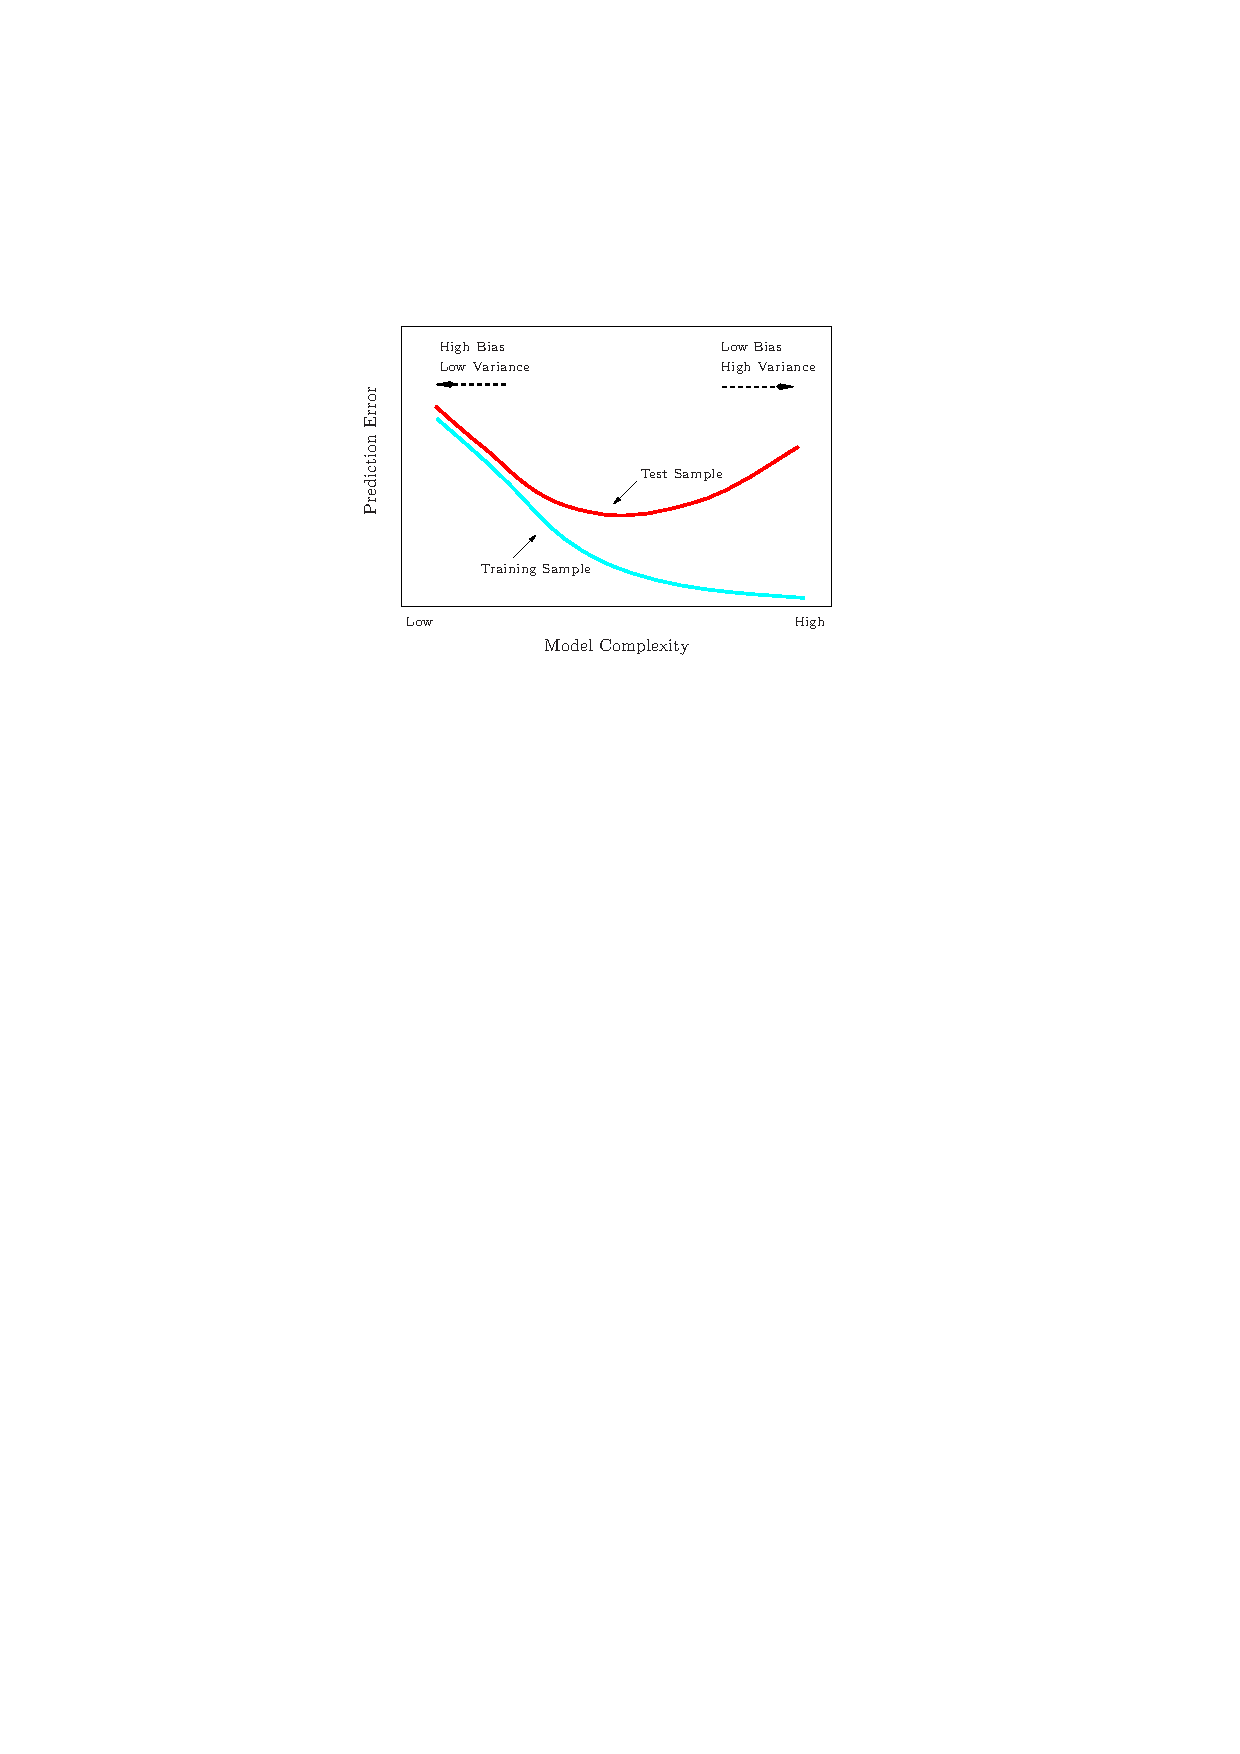
\includegraphics[width=.7\textwidth]{figures/tradeoff}
    \end{center}
  \end{overlayarea}

\end{frame}

\begin{frame}
  \frametitle{Linear regression}

  \begin{block}{Prediction error}
    For a fixed $\bX$, one has
   \begin{equation*}
      \hat{\mathrm{err}}(\bX \hatbbetaols)  = \sigma^2 \frac{(p+1)}{n} + \sigma^2.
    \end{equation*}
  \end{block}
  \vfill  
  
  \begin{block}{Gauss-Markov Theorem}
    $\hat Y = X^\intercal \hatbbetaols$ is the BLUE: the best model 
    (i.e. with the smallest variance) among unbiased estimators of 
    $\bbeta$.
  \end{block}
  \vfill

  $\rightsquigarrow$ Are  they some  cases where we  should \alert{\bf
    trade some bias for smaller variance} ?
\end{frame}

%%% Local Variables:
%%% mode: latex
%%% TeX-master: "slides.tex"
%%% End:


\subsection{Illustration: prostate cancer}



\begin{frame}[fragile]
  \frametitle{Example: prostate cancer data set}

  \begin{block}{The data set: 97 patient with prostate cancer}
    Examine  the  correlation  between  the level  of  cancer-specific
    antigen ($\mathbf{y}$) and various clinical measures.
  \end{block}

\begin{knitrout}\scriptsize
\definecolor{shadecolor}{rgb}{0.969, 0.969, 0.969}\color{fgcolor}\begin{kframe}
\begin{alltt}
\hlkwd{load}\hlstd{(}\hlstr{"prostate.rda"}\hlstd{)}
\hlstd{prostate} \hlopt \hlkwd{as_tibble}\hlstd{()} \hlopt \hlkwd{print}\hlstd{()}
\end{alltt}
\begin{verbatim}
## # A tibble: 97 x 10
##    lcavol lweight   age   lbph   svi   lcp gleason pgg45   lpsa train
##  *  <dbl>   <dbl> <int>  <dbl> <int> <dbl>   <int> <int>  <dbl> <lgl>
##  1 -0.580    2.77    50 -1.39      0 -1.39       6     0 -0.431 TRUE 
##  2 -0.994    3.32    58 -1.39      0 -1.39       6     0 -0.163 TRUE 
##  3 -0.511    2.69    74 -1.39      0 -1.39       7    20 -0.163 TRUE 
##  4 -1.20     3.28    58 -1.39      0 -1.39       6     0 -0.163 TRUE 
##  5  0.751    3.43    62 -1.39      0 -1.39       6     0  0.372 TRUE 
##  6 -1.05     3.23    50 -1.39      0 -1.39       6     0  0.765 TRUE 
##  7  0.737    3.47    64  0.615     0 -1.39       6     0  0.765 FALSE
##  8  0.693    3.54    58  1.54      0 -1.39       6     0  0.854 TRUE 
##  9 -0.777    3.54    47 -1.39      0 -1.39       6     0  1.05  FALSE
## 10  0.223    3.24    63 -1.39      0 -1.39       6     0  1.05  FALSE
## # ... with 87 more rows
\end{verbatim}
\end{kframe}
\end{knitrout}

\end{frame}

\begin{frame}[fragile]
  \frametitle{Correlations between predictors}

\begin{knitrout}\scriptsize
\definecolor{shadecolor}{rgb}{0.969, 0.969, 0.969}\color{fgcolor}\begin{kframe}
\begin{alltt}
\hlstd{prostate} \hlopt \hlkwd{filter}\hlstd{(train} \hlopt{==} \hlnum{TRUE}\hlstd{)} \hlopt \hlkwd{select}\hlstd{(}\hlopt{-}\hlstd{train)} \hlopt
  \hlkwd{ggpairs}\hlstd{(}\hlkwc{upper} \hlstd{=} \hlkwd{list}\hlstd{(}\hlkwc{continuous}\hlstd{=}\hlstr{"cor"}\hlstd{,}\hlkwc{combo}\hlstd{=}\hlstr{"box"}\hlstd{))}
\end{alltt}
\end{kframe}
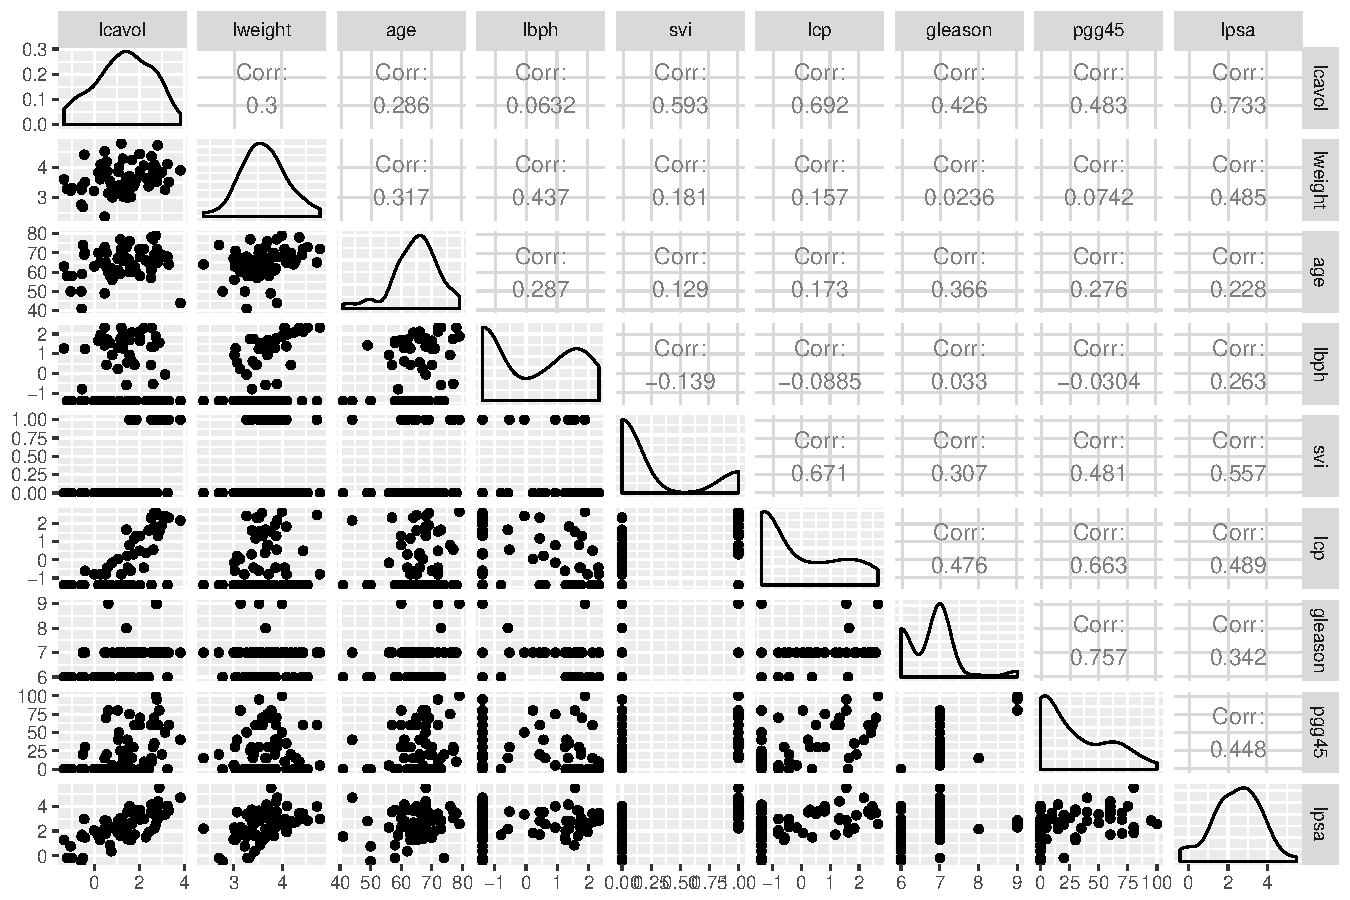
\includegraphics[width=.8\textwidth]{figures/plot_pairs-1} 

\end{knitrout}

\end{frame}

\begin{frame}[fragile]
  \frametitle{Correlations between predictors II}

\begin{knitrout}\scriptsize
\definecolor{shadecolor}{rgb}{0.969, 0.969, 0.969}\color{fgcolor}\begin{kframe}
\begin{alltt}
\hlstd{prostate} \hlopt
  \hlkwd{filter}\hlstd{(train} \hlopt{==} \hlnum{TRUE}\hlstd{)} \hlopt
  \hlkwd{select}\hlstd{(}\hlopt{-}\hlstd{train)} \hlopt
  \hlstd{cor} \hlopt \hlkwd{as.dist}\hlstd{()} \hlopt \hlkwd{print}\hlstd{()}
\end{alltt}
\begin{verbatim}
##              lcavol     lweight         age        lbph         svi
## lweight  0.30023199                                                
## age      0.28632427  0.31672347                                    
## lbph     0.06316772  0.43704154  0.28734645                        
## svi      0.59294913  0.18105448  0.12890226 -0.13914680            
## lcp      0.69204308  0.15682859  0.17295140 -0.08853456  0.67124021
## gleason  0.42641407  0.02355821  0.36591512  0.03299215  0.30687537
## pgg45    0.48316136  0.07416632  0.27580573 -0.03040382  0.48135774
## lpsa     0.73315515  0.48521519  0.22764238  0.26293763  0.55688643
##                 lcp     gleason       pgg45
## lweight                                    
## age                                        
## lbph                                       
## svi                                        
## lcp                                        
## gleason  0.47643684                        
## pgg45    0.66253335  0.75705650            
## lpsa     0.48920320  0.34242781  0.44804795
\end{verbatim}
\end{kframe}
\end{knitrout}

\end{frame}

\begin{frame}[fragile]
  \frametitle{Correlations between predictors III}

\begin{knitrout}\scriptsize
\definecolor{shadecolor}{rgb}{0.969, 0.969, 0.969}\color{fgcolor}\begin{kframe}
\begin{alltt}
\hlstd{prostate} \hlopt  \hlkwd{filter}\hlstd{(train} \hlopt{==} \hlnum{TRUE}\hlstd{)} \hlopt
  \hlkwd{select}\hlstd{(}\hlopt{-}\hlstd{train)} \hlopt \hlkwd{cor}\hlstd{()} \hlopt \hlkwd{corrplot}\hlstd{(}\hlkwc{method} \hlstd{=} \hlstr{"color"}\hlstd{,} \hlkwc{order} \hlstd{=} \hlstr{"hclust"}\hlstd{)}
\end{alltt}
\end{kframe}
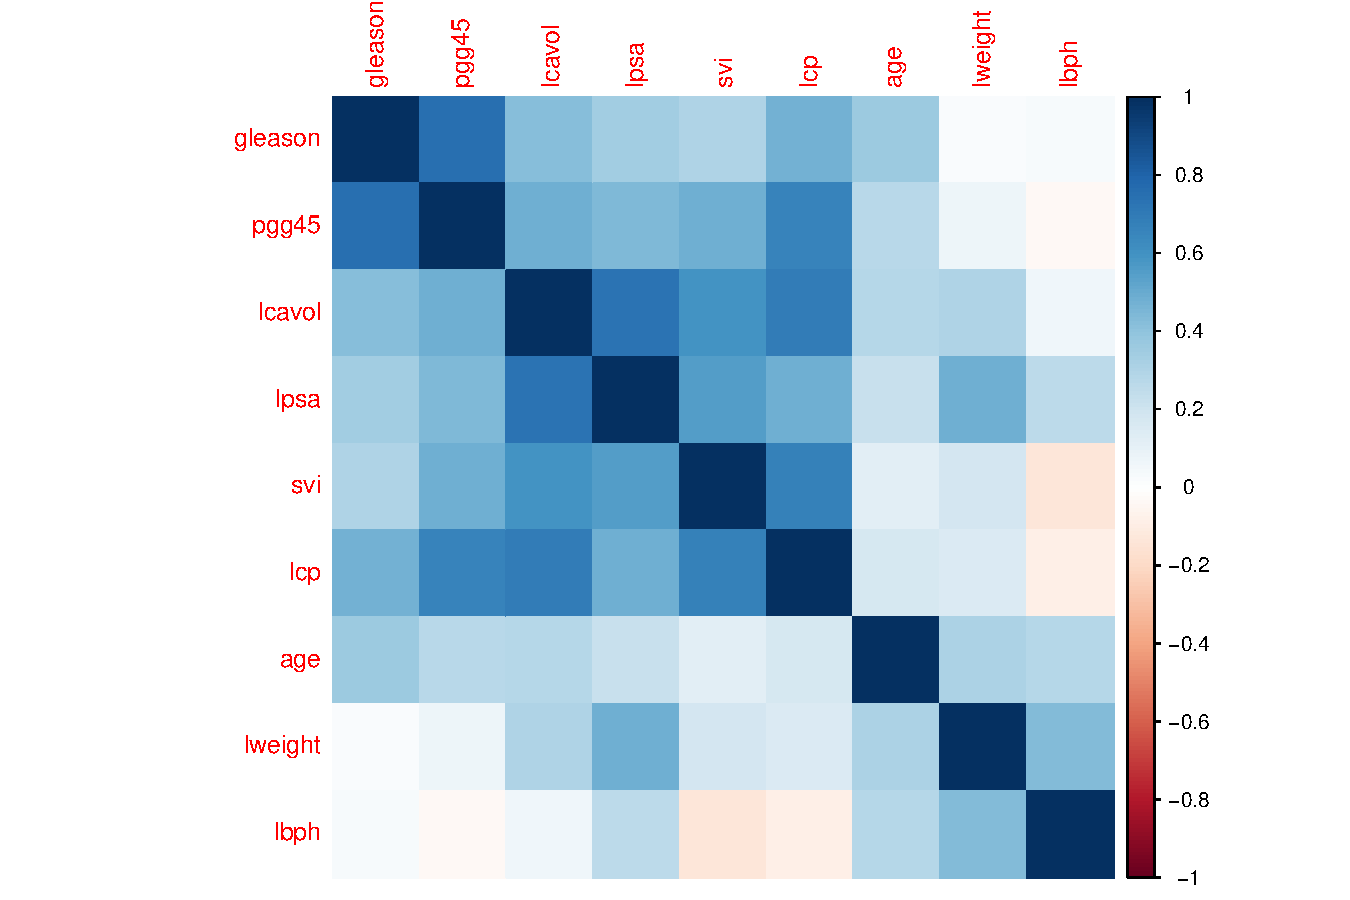
\includegraphics[width=.8\textwidth]{figures/plot_cor-1} 

\end{knitrout}

\end{frame}


\begin{frame}[containsverbatim,allowframebreaks]
  \frametitle{OLS and limitations}

For studying the correlation effect, we normalize and create test and train sets
\begin{knitrout}\scriptsize
\definecolor{shadecolor}{rgb}{0.969, 0.969, 0.969}\color{fgcolor}\begin{kframe}
\begin{alltt}
\hlstd{prostate_train} \hlkwb{<-}
  \hlstd{prostate} \hlopt \hlkwd{filter}\hlstd{(train} \hlopt{==} \hlnum{TRUE}\hlstd{)}  \hlopt \hlkwd{select}\hlstd{(}\hlopt{-}\hlstd{train)} \hlopt
  \hlkwd{scale}\hlstd{(}\hlnum{FALSE}\hlstd{,} \hlnum{TRUE}\hlstd{)} \hlopt \hlkwd{as_data_frame}\hlstd{()}
\hlstd{prostate_test}  \hlkwb{<-}
  \hlstd{prostate} \hlopt \hlkwd{filter}\hlstd{(train} \hlopt{==} \hlnum{FALSE}\hlstd{)} \hlopt \hlkwd{select}\hlstd{(}\hlopt{-}\hlstd{train)} \hlopt
  \hlkwd{scale}\hlstd{(}\hlnum{FALSE}\hlstd{,} \hlnum{TRUE}\hlstd{)} \hlopt \hlkwd{as_data_frame}\hlstd{()}
\hlstd{model.full} \hlkwb{<-} \hlkwd{lm}\hlstd{(lpsa}\hlopt{~}\hlstd{., prostate_train)}
\end{alltt}
\end{kframe}
\end{knitrout}

   \begin{block}{Estimating prediction error}
  \end{block}
\begin{knitrout}\scriptsize
\definecolor{shadecolor}{rgb}{0.969, 0.969, 0.969}\color{fgcolor}\begin{kframe}
\begin{alltt}
\hlstd{y_hat} \hlkwb{<-} \hlkwd{predict}\hlstd{(model.full,} \hlkwc{newdata}\hlstd{=prostate_test)}
\hlstd{y_test} \hlkwb{<-} \hlstd{prostate_test}\hlopt{$}\hlstd{lpsa}
\hlstd{err_ols} \hlkwb{<-} \hlkwd{mean}\hlstd{((y_test}\hlopt{-}\hlstd{y_hat)}\hlopt{^}\hlnum{2}\hlstd{)}
\hlkwd{print}\hlstd{(err_ols)}
\end{alltt}
\begin{verbatim}
## [1] 0.0673631
\end{verbatim}
\end{kframe}
\end{knitrout}

\begin{knitrout}\tiny
\definecolor{shadecolor}{rgb}{0.969, 0.969, 0.969}\color{fgcolor}\begin{kframe}
\begin{alltt}
\hlkwd{summary}\hlstd{(model.full)}
\end{alltt}
\begin{verbatim}
## 
## Call:
## lm(formula = lpsa ~ ., data = prostate_train)
## 
## Residuals:
##      Min       1Q   Median       3Q      Max 
## -0.59947 -0.12416 -0.01972  0.16341  0.54059 
## 
## Coefficients:
##             Estimate Std. Error t value Pr(>|t|)    
## (Intercept)  0.15605    0.56489   0.276  0.78334    
## lcavol       0.38055    0.07092   5.366 1.47e-06 ***
## lweight      0.82258    0.29903   2.751  0.00792 ** 
## age         -0.45367    0.32500  -1.396  0.16806    
## lbph         0.07718    0.03754   2.056  0.04431 *  
## svi          0.12779    0.05175   2.469  0.01651 *  
## lcp         -0.10632    0.05695  -1.867  0.06697 .  
## gleason     -0.07315    0.49870  -0.147  0.88389    
## pgg45        0.13589    0.07820   1.738  0.08755 .  
## ---
## Signif. codes:  0 '***' 0.001 '**' 0.01 '*' 0.05 '.' 0.1 ' ' 1
## 
## Residual standard error: 0.259 on 58 degrees of freedom
## Multiple R-squared:  0.6944,	Adjusted R-squared:  0.6522 
## F-statistic: 16.47 on 8 and 58 DF,  p-value: 2.042e-12
\end{verbatim}
\end{kframe}
\end{knitrout}
\end{frame}

\begin{frame}
  \frametitle{Comments}

  Why do  some coefficients in  $\bbeta$ are not well  estimated/ have
  large variance? (pgg45, gleason)

  \begin{block}{Statistical issue}
    \alert{Correlated variables are not well estimated},\\
    
    \rsa  they carry the same information regarding the response.

  \end{block}

  \vfill

  \begin{block}{Numerical issue}
    \alert{Correlated variables leads to bad conditioning of $\bX^T\bX$},\\

    \rsa OLS cannot be computed  when they are redundant variables in
      $\bX$ \alert{or when $n<p$}.
  \end{block}
  
  $\rightsquigarrow$ \textit{interpretation becomes rather difficult}

\end{frame}

\begin{frame}
  \frametitle{Solutions}

  \begin{block}{Variable selection}
    If the  underlying model  is assumed to  have only  few predictors
    truly related to the outcome,  we may want to \alert{select} those
    with the highest effect. We are looking for both
    \begin{itemize}
    \item better interpretability.
    \item better predictive performances.
    \end{itemize}
  \end{block}

  \vfill

  \begin{block}{Regularization}
    If  all  the predictors  have  similar  or  close effects  on  the
    response, selection (and thus interpretability) is out of reach.

    We may \alert{regularize} the problem by \alert{constraining} the
    parameters $\bbeta$ to  live in an appropriate set  that will make
    the $\bX^T\bX$ invertible.
  \end{block}

\end{frame}
 
\section{Variable Selection}
 

\begin{frame}
  \frametitle{Variable Selection}

  \begin{block}{Problematic}
    
  With many regressor, 
  \begin{itemize}
  \item we integrate more and more information in the model ;
  \item we have more and more parameters to estimate and $\var (\hat{Y}_i)\nearrow$.
  \end{itemize}  
\end{block}

  \vfill
  
  \begin{block}{Idea}
    Look for a (small)  set $\mathcal{S}$ with  $k$ variables
    among $p$ such that
  \begin{equation*}
    Y \approx X_{\mathcal{S}}^T \hatbbeta_{\mathcal{S}}.
  \end{equation*} 
    \end{block}

  \begin{block}{Ingredients}
    To find this tradeoff, we need
    \begin{enumerate}
    \item a \alert{criterion} to evaluate the performance ;
    \item an \alert{algorithm} to determine the subset of $k$ variables optimising the criterion.
    \end{enumerate}
  \end{block}

\end{frame}

\subsection{Criteria for model comparison}

\begin{frame}
  \frametitle{Estimation of the prediction error by cross-validation}
  \framesubtitle{For the regression: PRESS (\textit{predicted residual sum of squares})}

  \begin{block}{Principe}
    \vspace{-.25cm}
    \begin{enumerate}
    \item Split the data into $K$ subsets,
    \item Successively use each subset as the test set,
    \item Compute the test error for the $K$ subsets,
    \item Average the $K$ error to get the final estiamte.
    \end{enumerate}
  \end{block}

  \vspace{-.25cm}
  
  \begin{block}{Formalism}
    Let  $\kappa  :  \{1,\dots,n\} \rightarrow  \{1,\dots,K\}$  be  an
    indexing   function  that   indicates  the   partition  to   which
    observation  $i$   is  allocated   by  randomization.   Denote  by
    $\hat{f}^{-\kappa(i)}$ the  fitted model, computed with  the $k$th
    part of the data removed.  Then
   \begin{equation*}
     \mathrm{CV}(\hat{\bbeta})     =    \frac{1}{n}\sum_{i=1}^n
     (y_i - x_i^T \hat{\bbeta}^{-\kappa(i)} )^2
   \end{equation*}
   provides an estimate of the prediction error.
  \end{block}
  
\end{frame}

\begin{frame}
  \frametitle{Penalized Criterion}
  \framesubtitle{Principle}
  
  \begin{block}{Idea}
    Rather than estimating the prediciton error with the test error, we estimate how much the training error under estimate the true prediction error.
  \end{block}

  \vfill
  
  \begin{block}{General form}
   Based on the available model fit, compute
    \begin{equation*}
      \hat{\mathrm{err}} = \mathrm{err}_{\mathcal{D}} + \mathrm{"optimism"}.
    \end{equation*}
  \end{block}

  \vfill
  
  \begin{block}{Remarks}
    \begin{itemize}
    \item \og penalize \fg to much complex models
    \end{itemize}
  \end{block}

\end{frame}

\begin{frame}
  \frametitle{Penalized Criteria}
  \framesubtitle{The most Popular in linear regression}

    Let $k$ be the size of the current model (i.e. the current number of predictors).
    
    \vfill

    \begin{block}{Criterion for the Linear regression model
        \only<1>{$\sigma$ known}\only<2>{$\sigma$ unknown}}
      We choose  the model with size  $k$ minimizing one of the following
      \begin{itemize}
    \item      \alert{\bf      Aka\"ike     Information      Criteria}
      \only<1>{equivalent to $C_p$ when $\sigma$ is known} \only<2>{$\sigma^2$ estimated by $\err_{\mathcal{D}}/n$}
      \[ 
      \mathrm{AIC} = - 2 \mathrm{loglik} + 2 k
      \only<1>{ = \frac{n}{\sigma^2} \mathrm{err}_{\mathcal{D}} + 2 k .}
      \only<2>{ = n \log(\mathrm{err}_{\mathcal{D}}) + 2 k .}
      \]
      
    \item \alert{\bf Bayesian Information Criterion} \only<2>{$\sigma^2$ estimated by $\err_{\mathcal{D}}/n$}
      \[ 
      \mathrm{BIC} = - 2 \mathrm{loglik} + k \log(n)
      \only<1>{ = \frac{n}{\sigma^2} \mathrm{err}_{\mathcal{D}} + k \log(n) .}
      \only<2>{ = n \log(\mathrm{err}_{\mathcal{D}}) + k \log(n) .}
      \]
    \end{itemize}
    \end{block}
  
\end{frame}

% \begin{frame}{$C_p$/AIC: proof}
% 
% Ideally, we would like to minimize the error of the mean distance between the true model $\bX  \bbeta =  \bmu$  and the OLS. This diustance splits as follows
% \begin{align*}
% \| \bmu - \bX \hatbbetaols \|^2 = & \| \by - \varepsilon - \bP_\bX \by \|^2 \\
%  =& \| \by -  \hat\by \|^2 + \| \varepsilon \|^2  -2 \varepsilon^\intercal (\by -\bP_\bX\by) \\
%   = & n \err_{\mathcal{D}}  + \| \varepsilon  \|^2 -2 \varepsilon^\intercal  (\bI -\bP_\bX) (\bmu + \varepsilon)\\
%   = & n\err_{\mathcal{D}} - \| \varepsilon \|^2 +2 \varepsilon^\intercal \bP_\bX \varepsilon -2
% \varepsilon^\intercal (\bI -\bP_\bX) \bmu
% \end{align*}
% 
% On average we get
% \begin{itemize}
% \item $\E[\| \varepsilon \|^2] = n \sigma^2$
% \item $\E[\varepsilon^\intercal (\bI-\bP_\bX)\bmu]=0$
% \item $\E[2 \varepsilon^\intercal \bP_\bX \varepsilon]= 2 \E[ \trace{\varepsilon^\intercal \bP_\bX
%   \varepsilon}]=2 \trace{\bP_\bX}\sigma^2$
% \end{itemize}
% 
% If $k$ is the dimension of the space of the projection, we find
% $$
% \E \| \bmu - \bX \hatbbetaols \|^2 = n \err_{\mathcal{D}} - n \sigma^2 +2 k \sigma^2
% $$
% We then just have to divide by $n \sigma^2$.
% \end{frame}

\subsection{Algorithms for variable subset selection}

\begin{frame}
  \frametitle{Exhaustive search  (best-subset)}

  \begin{block}{Algorithm}
    For $k=0,\dots,p$,  find the subset with  $k$ variables with the smallest  $SCR$ among $2^k$ models.
  \end{block}
  
  \vfill
  
  \begin{block}{Properties}
    \begin{itemize}
    \item Generalize to any criterion ($R^2$, AIC, BIC\dots)
    \item Efficient algorithm with pruning  (\og Leaps and Bound \fg)
    \item impossible as soon as $p>30$.
    \end{itemize}
  \end{block}
\end{frame}

\begin{frame}
  \frametitle{\only<1>{(Forward regression)} \only<2>{Forward-stepwise}}

  \begin{block}{Algorithm}
    \begin{itemize}
    \item[1.] Begin with $\mathcal{S} = \emptyset$
    \item[2.]<1> at step $k$ find the variable which, added to $\mathcal{S}$, 
      gives the best model
    \item[2'.]<2> At step $k$ find the best model by either adding or removing one variable.
    \item[3] etc. until $p$ variables enter the model
      
    \end{itemize}
  \end{block}
  
  \vfill
  
  \begin{block}{Properties}
    \begin{itemize}
    \item Best model is understood asadjusted $R^2$, AIC, BIC\dots
    \item useful when $p$ is large
    \item large bias, but variance/complexity controlled.
    \item \og greedy \fg\ algorithm
    \end{itemize}
  \end{block}

\end{frame}

% \begin{frame}
%   \frametitle{Backward regression}
% 
%   \begin{block}{Algorithm}
%     \begin{enumerate}
%     \item[1] Start with the full model $\mathcal{S} = \set{1,\dots,p}$
%     \item[2]  At step    $k$,  remove the less influent   variable.
%     \item[3] etc. until $\mathcal{S}$ is empty.
%     \end{enumerate}
%   \end{block}
%   
%   \vfill
%   
%   \begin{block}{Properties}
%     \begin{itemize}
%     \item Best model is understood as SCR or $R^2$,
%       AIC, BIC\dots
%     \item does not work  when $n < p$
%     \item large bias, but variance/complexity controlled.
%     \item \og greedy \fg\ algorithm
%     \end{itemize}
%   \end{block}
% 
% \end{frame}
% 
 

\subsection{Illustration: prostate cancer}



\begin{frame}[containsverbatim,allowframebreaks]
  \frametitle{Exhaustive search}

\begin{knitrout}\scriptsize
\definecolor{shadecolor}{rgb}{0.969, 0.969, 0.969}\color{fgcolor}\begin{kframe}
\begin{alltt}
\hlkwd{library}\hlstd{(leaps)}
\end{alltt}
\end{kframe}
\end{knitrout}

Get all possible models
\begin{knitrout}\scriptsize
\definecolor{shadecolor}{rgb}{0.969, 0.969, 0.969}\color{fgcolor}\begin{kframe}
\begin{alltt}
\hlstd{out} \hlkwb{<-} \hlkwd{regsubsets}\hlstd{(}
          \hlstd{lpsa} \hlopt{~} \hlstd{. ,}
          \hlkwc{data}  \hlstd{= prostate_train,}
          \hlkwc{nbest} \hlstd{=} \hlnum{100}\hlstd{,}
          \hlkwc{really.big} \hlstd{=} \hlnum{TRUE}
        \hlstd{)}
\hlstd{bss} \hlkwb{<-} \hlkwd{summary}\hlstd{(out)}
\end{alltt}
\end{kframe}
\end{knitrout}

Extract size and RSS. Add the null model (with just the intercept)
\begin{knitrout}\scriptsize
\definecolor{shadecolor}{rgb}{0.969, 0.969, 0.969}\color{fgcolor}\begin{kframe}
\begin{alltt}
\hlstd{intercept} \hlkwb{<-} \hlkwd{lm}\hlstd{(lpsa} \hlopt{~} \hlnum{1}\hlstd{,} \hlkwc{data} \hlstd{= prostate_train)}
\end{alltt}
\end{kframe}
\end{knitrout}


\end{frame}

\begin{frame}
  \frametitle{Exhaustive search II}
\begin{knitrout}\scriptsize
\definecolor{shadecolor}{rgb}{0.969, 0.969, 0.969}\color{fgcolor}
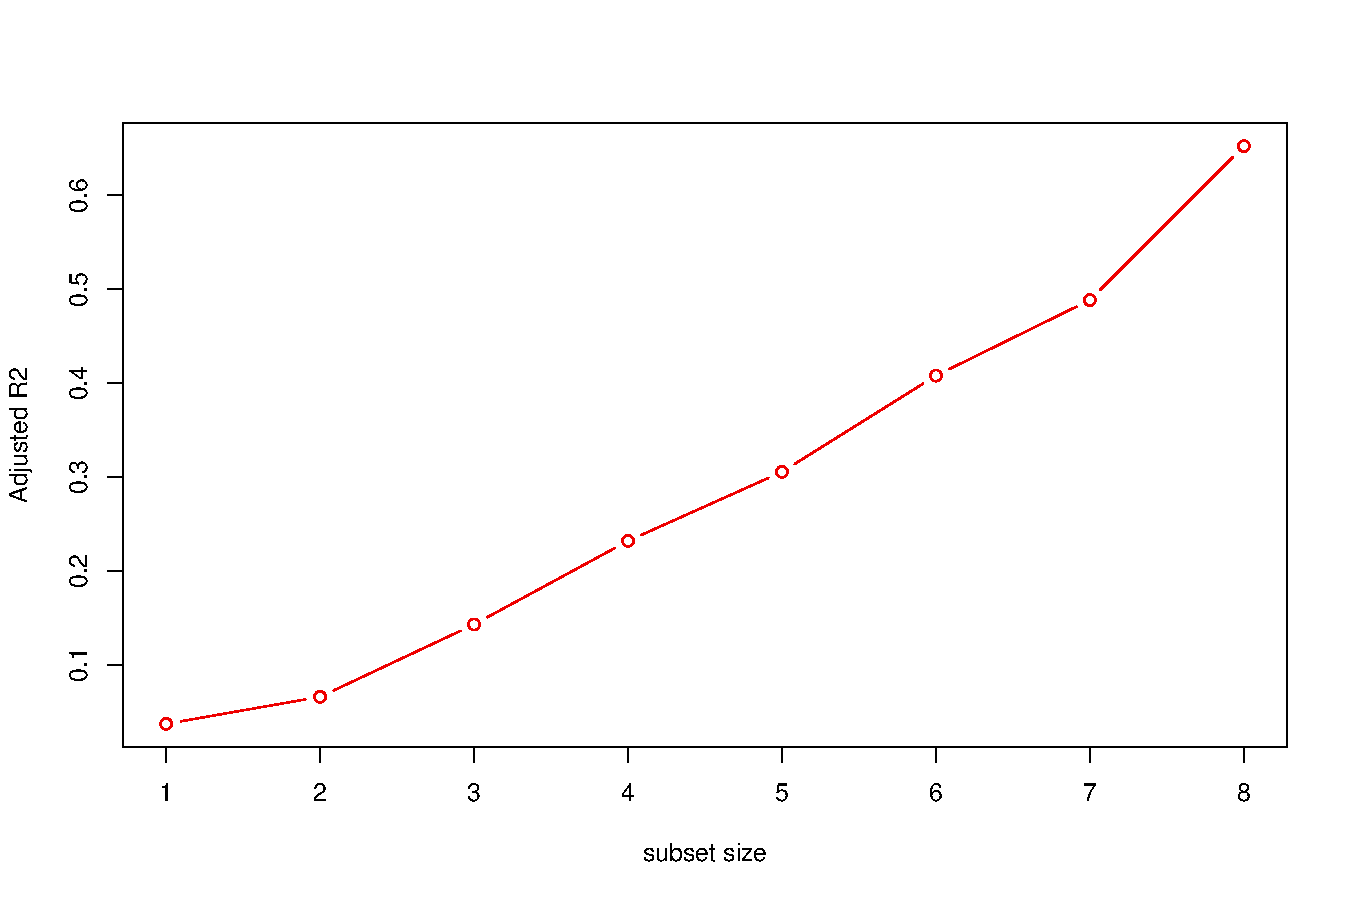
\includegraphics[width=.8\textwidth]{figures/bss_r2-1} 

\end{knitrout}
\end{frame}

\begin{frame}
  \frametitle{Exhaustive search III}
\begin{knitrout}\scriptsize
\definecolor{shadecolor}{rgb}{0.969, 0.969, 0.969}\color{fgcolor}
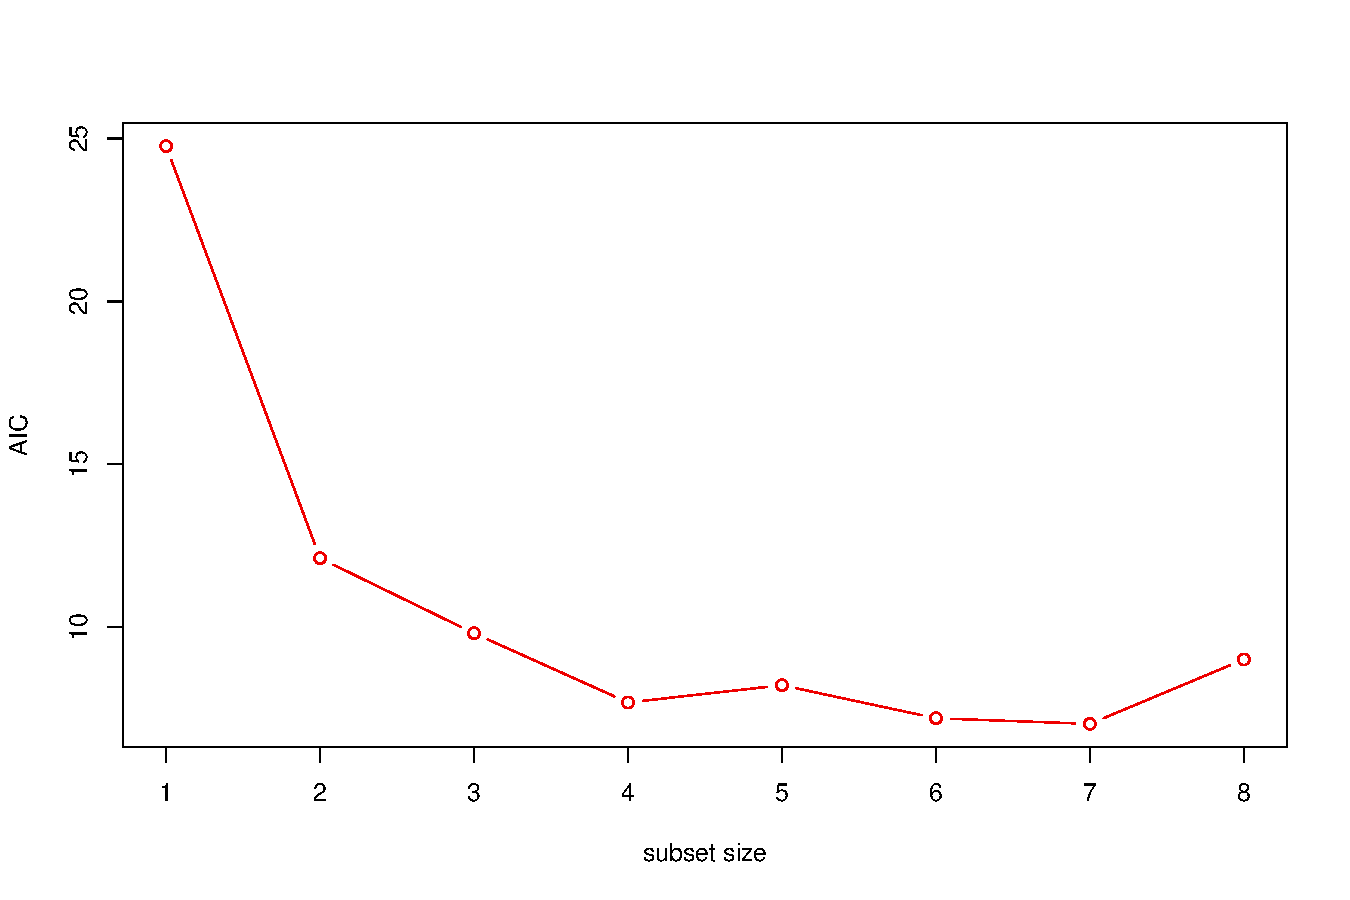
\includegraphics[width=.8\textwidth]{figures/bss_AIC-1} 

\end{knitrout}
\end{frame}

\begin{frame}
  \frametitle{Exhaustive search IV}

\begin{knitrout}\scriptsize
\definecolor{shadecolor}{rgb}{0.969, 0.969, 0.969}\color{fgcolor}
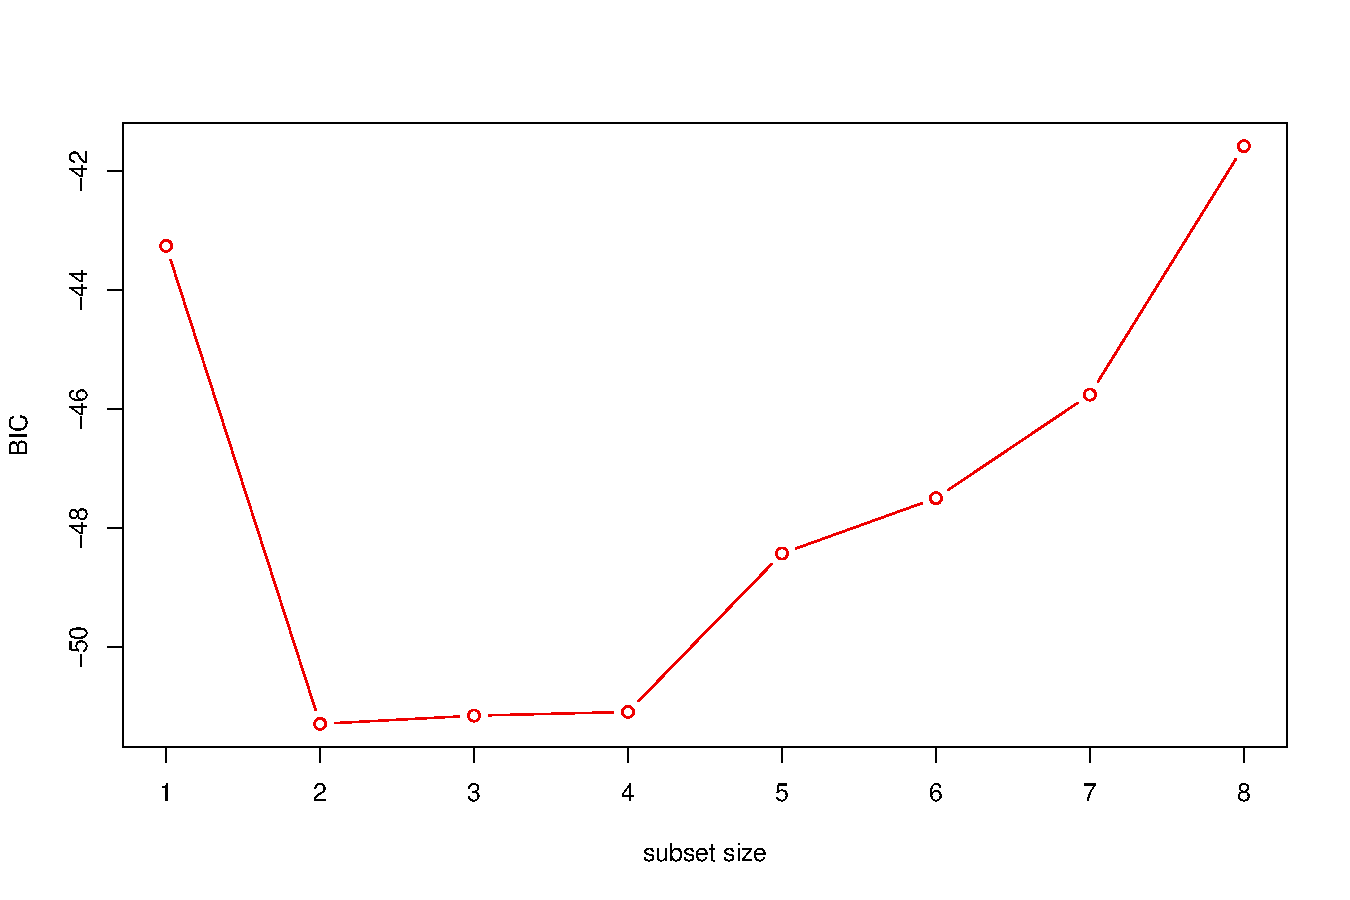
\includegraphics[width=.8\textwidth]{figures/bss_BIC-1} 

\end{knitrout}

\end{frame}

\begin{frame}[containsverbatim]
  \frametitle{Forward-Stepwise (I)}

Create the nul model and the full model
\begin{knitrout}\scriptsize
\definecolor{shadecolor}{rgb}{0.969, 0.969, 0.969}\color{fgcolor}\begin{kframe}
\begin{alltt}
\hlstd{null}  \hlkwb{<-} \hlkwd{lm}\hlstd{(lpsa} \hlopt{~} \hlnum{1}\hlstd{,} \hlkwc{data} \hlstd{= prostate_train)}
\hlstd{full}  \hlkwb{<-} \hlkwd{lm}\hlstd{(lpsa} \hlopt{~} \hlstd{.,} \hlkwc{data} \hlstd{= prostate_train)}
\end{alltt}
\end{kframe}
\end{knitrout}

Create the scope of models
\begin{knitrout}\scriptsize
\definecolor{shadecolor}{rgb}{0.969, 0.969, 0.969}\color{fgcolor}\begin{kframe}
\begin{alltt}
\hlstd{lower} \hlkwb{<-} \hlopt{~}\hlnum{1}
\hlstd{upper} \hlkwb{<-} \hlopt{~}\hlstd{lcavol}\hlopt{+}\hlstd{lweight}\hlopt{+}\hlstd{age}\hlopt{+}\hlstd{lbph}\hlopt{+}\hlstd{svi}\hlopt{+}\hlstd{lcp}\hlopt{+}\hlstd{gleason}\hlopt{+}\hlstd{pgg45}
\hlstd{scope} \hlkwb{<-} \hlkwd{list}\hlstd{(}\hlkwc{lower} \hlstd{= lower,}\hlkwc{upper} \hlstd{= upper)}
\end{alltt}
\end{kframe}
\end{knitrout}

Stepwise with AIC: forward, backward, both
\begin{knitrout}\scriptsize
\definecolor{shadecolor}{rgb}{0.969, 0.969, 0.969}\color{fgcolor}\begin{kframe}
\begin{alltt}
\hlstd{fwd}  \hlkwb{<-} \hlkwd{step}\hlstd{(null, scope,} \hlkwc{direction} \hlstd{=} \hlstr{"forward"} \hlstd{,} \hlkwc{trace}\hlstd{=}\hlnum{FALSE}\hlstd{)}
\hlstd{bwd}  \hlkwb{<-} \hlkwd{step}\hlstd{(full, scope,} \hlkwc{direction} \hlstd{=} \hlstr{"backward"}\hlstd{,} \hlkwc{trace}\hlstd{=}\hlnum{FALSE}\hlstd{)}
\hlstd{both} \hlkwb{<-} \hlkwd{step}\hlstd{(null, scope,} \hlkwc{direction} \hlstd{=} \hlstr{"both"}   \hlstd{,} \hlkwc{trace}\hlstd{=}\hlnum{FALSE}\hlstd{)}
\end{alltt}
\end{kframe}
\end{knitrout}

\vfill

\rsa 3  equivalent models
\end{frame}

\begin{frame}[containsverbatim]
  \frametitle{Forward regression}

\begin{scriptsize}
\begin{knitrout}\scriptsize
\definecolor{shadecolor}{rgb}{0.969, 0.969, 0.969}\color{fgcolor}\begin{kframe}
\begin{alltt}
\hlstd{fwd}
\end{alltt}
\begin{verbatim}
## 
## Call:
## lm(formula = lpsa ~ lcavol + lweight + svi + lbph, data = prostate_train)
## 
## Coefficients:
## (Intercept)       lcavol      lweight          svi         lbph  
##     -0.1185       0.3337       0.7219       0.1165       0.0746
\end{verbatim}
\begin{alltt}
\hlstd{fwd}\hlopt{$}\hlstd{anova}
\end{alltt}
\begin{verbatim}
##        Step Df  Deviance Resid. Df Resid. Dev       AIC
## 1           NA        NA        66  12.729028 -109.2741
## 2  + lcavol -1 6.8420623        65   5.886966 -158.9408
## 3 + lweight -1 0.9831846        64   4.903781 -169.1840
## 4     + svi -1 0.2887517        63   4.615030 -171.2501
## 5    + lbph -1 0.2766756        62   4.338354 -173.3922
\end{verbatim}
\end{kframe}
\end{knitrout}
\end{scriptsize}
  
\end{frame}

\begin{frame}[containsverbatim]
  \frametitle{Backward regression}

\begin{scriptsize}
\begin{knitrout}\scriptsize
\definecolor{shadecolor}{rgb}{0.969, 0.969, 0.969}\color{fgcolor}\begin{kframe}
\begin{alltt}
\hlstd{bwd}
\end{alltt}
\begin{verbatim}
## 
## Call:
## lm(formula = lpsa ~ lcavol + lweight + age + lbph + svi + lcp + 
##     pgg45, data = prostate_train)
## 
## Coefficients:
## (Intercept)       lcavol      lweight          age         lbph  
##     0.09420      0.37883      0.82953     -0.46510      0.07695  
##         svi          lcp        pgg45  
##     0.12858     -0.10586      0.12842
\end{verbatim}
\begin{alltt}
\hlstd{bwd}\hlopt{$}\hlstd{anova}
\end{alltt}
\begin{verbatim}
##        Step Df    Deviance Resid. Df Resid. Dev       AIC
## 1           NA          NA        58   3.890358 -172.6948
## 2 - gleason  1 0.001443147        59   3.891801 -174.6700
\end{verbatim}
\end{kframe}
\end{knitrout}
\end{scriptsize}

\end{frame}
\begin{frame}[containsverbatim]
  \frametitle{Stepwise regression}

\begin{scriptsize}
\begin{knitrout}\scriptsize
\definecolor{shadecolor}{rgb}{0.969, 0.969, 0.969}\color{fgcolor}\begin{kframe}
\begin{alltt}
\hlstd{both}
\end{alltt}
\begin{verbatim}
## 
## Call:
## lm(formula = lpsa ~ lcavol + lweight + svi + lbph, data = prostate_train)
## 
## Coefficients:
## (Intercept)       lcavol      lweight          svi         lbph  
##     -0.1185       0.3337       0.7219       0.1165       0.0746
\end{verbatim}
\begin{alltt}
\hlstd{both}\hlopt{$}\hlstd{anova}
\end{alltt}
\begin{verbatim}
##        Step Df  Deviance Resid. Df Resid. Dev       AIC
## 1           NA        NA        66  12.729028 -109.2741
## 2  + lcavol -1 6.8420623        65   5.886966 -158.9408
## 3 + lweight -1 0.9831846        64   4.903781 -169.1840
## 4     + svi -1 0.2887517        63   4.615030 -171.2501
## 5    + lbph -1 0.2766756        62   4.338354 -173.3922
\end{verbatim}
\end{kframe}
\end{knitrout}
\end{scriptsize}
  
\end{frame}

\begin{frame}[fragile]
  \frametitle{Performance on test data}

\begin{knitrout}\scriptsize
\definecolor{shadecolor}{rgb}{0.969, 0.969, 0.969}\color{fgcolor}\begin{kframe}
\begin{alltt}
\hlkwd{print}\hlstd{(err_ols)}
\end{alltt}
\begin{verbatim}
## [1] 0.0673631
\end{verbatim}
\begin{alltt}
\hlkwd{print}\hlstd{(err_AIC.fwd}  \hlkwb{<-} \hlkwd{mean}\hlstd{((y_test} \hlopt{-} \hlkwd{predict}\hlstd{(fwd , prostate_test))}\hlopt{^}\hlnum{2}\hlstd{))}
\end{alltt}
\begin{verbatim}
## [1] 0.05838145
\end{verbatim}
\begin{alltt}
\hlkwd{print}\hlstd{(err_AIC.bwd}  \hlkwb{<-} \hlkwd{mean}\hlstd{((y_test} \hlopt{-} \hlkwd{predict}\hlstd{(bwd , prostate_test))}\hlopt{^}\hlnum{2}\hlstd{))}
\end{alltt}
\begin{verbatim}
## [1] 0.06680086
\end{verbatim}
\begin{alltt}
\hlkwd{print}\hlstd{(err_AIC} \hlkwb{<-} \hlkwd{mean}\hlstd{((y_test} \hlopt{-} \hlkwd{predict}\hlstd{(both, prostate_test))}\hlopt{^}\hlnum{2}\hlstd{))}
\end{alltt}
\begin{verbatim}
## [1] 0.05838145
\end{verbatim}
\end{kframe}
\end{knitrout}

\end{frame}


\begin{frame}[containsverbatim]
  \frametitle{Stepwise: BIC modification}
  \framesubtitle{More sparse model}
  
\begin{knitrout}\scriptsize
\definecolor{shadecolor}{rgb}{0.969, 0.969, 0.969}\color{fgcolor}\begin{kframe}
\begin{alltt}
\hlstd{BIC} \hlkwb{<-} \hlkwd{step}\hlstd{(null, scope,} \hlkwc{k} \hlstd{=} \hlkwd{log}\hlstd{(n} \hlkwb{<-} \hlkwd{nrow}\hlstd{(prostate)),} \hlkwc{trace}\hlstd{=}\hlnum{FALSE}\hlstd{)}
\hlstd{BIC}
\end{alltt}
\begin{verbatim}
## 
## Call:
## lm(formula = lpsa ~ lcavol + lweight, data = prostate_train)
## 
## Coefficients:
## (Intercept)       lcavol      lweight  
##     -0.3816       0.4143       0.9892
\end{verbatim}
\begin{alltt}
\hlkwd{print}\hlstd{(err_BIC}  \hlkwb{<-} \hlkwd{mean}\hlstd{((y_test} \hlopt{-} \hlkwd{predict}\hlstd{(BIC, prostate_test))}\hlopt{^}\hlnum{2}\hlstd{))}
\end{alltt}
\begin{verbatim}
## [1] 0.06342134
\end{verbatim}
\end{kframe}
\end{knitrout}
\end{frame}


\begin{frame}
  \frametitle{Comments}

  \begin{block}{Interpretability}
    \begin{enumerate}
    \item If the true $\mathcal{S}$ only contains a  \alert{\bf few
      variables linked to the response},\\
      $\rightsquigarrow$ variable selection algorithms can retrieve relevent predictors.
    \item  If the true   $\mathcal{S}$  contains  \alert{\bf many correlated predictors}\\
      $\rightsquigarrow$  the selected variables will be hardly interpretable.
    \end{enumerate}
  \end{block}

  \vfill

  \begin{block}{Stability issue}
    With strong correlation or when $n < p$, \alert{\bf small changes} in the data can induce   \alert{\bf large discrepencies }  between the sets of selected variables.
   \end{block}

\end{frame}

\section{Regularisation}
 

\subsection{Motivations et principle}

\begin{frame}
  \frametitle{Several goals}

  Control the parameter $\hatbbeta$ to

  \begin{enumerate}
  \item \alert{Regularize} the problem
    \begin{itemize}
    \item For numerical purpose, (conditioning of $\bX^T\bX$),
    \item     For    stability    purpose,     (correlation    between
      $(X_1,\dots,X_p)$).
    \end{itemize}
  \item \alert{Enhance} the prediction
    \begin{itemize}
    \item By trading a little bias vs variance
    \item By controlling irrelevant variables
    \end{itemize}
  \item \alert{Looking towards} interpretability
    \begin{itemize}
    \item By controlling model complexity,
    \item By embedding the variable selection (Lasso).
    \end{itemize}
  \end{enumerate}

\end{frame}

\pgfdeclareimage[height=0.8\textheight]{sparsity1}{figures/sparsity_1}
\pgfdeclareimage[height=0.8\textheight]{sparsity2}{figures/sparsity_2}
\pgfdeclareimage[height=0.375\textheight]{sparsity4}{figures/sparsity_4}

%--------------------------------------%
\begin{frame}
  \frametitle{A Geometric View of Shrinkage}
  \framesubtitle{Constrained Optimization}

  \begin{overlayarea}{\textwidth}{\textheight}
    \begin{columns}
      \begin{column}{0.475\textwidth}
        \begin{tikzpicture}
          \only<1>{%
            \node (Surf) at (0,0) {\pgfuseimage{sparsity1}}
            node     at    (Surf.west)    [rotate=90,yshift=5mm]
            {$L(\beta_1,\beta_2;\mathbf{X})$}
            node at (Surf.south west) [xshift=5mm,yshift=5mm]{$\beta_2$}
            node at (Surf.south east) [xshift=-7.5mm,yshift=2.5mm]{$\beta_1$};
          }
          \only<2>{%
            \node (Surf2) at (0,0) {\pgfuseimage{sparsity2}}
            node    at    (Surf2.west)    [rotate=90,yshift=5mm]
            {$L(\beta_1,\beta_2;\mathbf{X})$}
            node at (Surf2.south west) [xshift=5mm,yshift=5mm]{$\beta_2$}
            node at (Surf2.south east) [xshift=-7.5mm,yshift=2.5mm]{$\beta_1$};
          }
          \only<3->{%
            \node (titi) at (0,0) {\phantom{titi}};
            \node (Surf3) at (0,-4.5) {\pgfuseimage{sparsity4}}
            node at (Surf3.west) [rotate=90,yshift=2.5mm] {$\beta_2$}
            node at (Surf3.south) [yshift=-2.5mm] {$\beta_1$};
          }
        \end{tikzpicture}
      \end{column}
      \begin{column}{0.55\textwidth}
        \only<1>{%
          We basically want to solve a problem of the form
          \begin{equation*}
            \maximize_{\beta_1,\beta_2} L(\beta_1,\beta_2;\mathbf{X})
          \end{equation*}
          where $L$ is typically a concave likelihood function.

          This is strictly equivalent to solve
          \begin{equation*}
            \minimize_{\beta_1,\beta_2} L'(\beta_1,\beta_2;\mathbf{X})
          \end{equation*}
          where $L'=-L$ is convex ! For instance the squared error loss in the
          OLS.
        }
        \only<2->{%
          \begin{equation*}
            \left\{\begin{array}{ll}
                \displaystyle    \maximize_{\beta_1,\beta_2}   &
                L(\beta_1,\beta_2;\mathbf{X})\\
                \mathrm{s.t.} & \Omega(\beta_1,\beta_2) \leq c
              \end{array}\right.,
          \end{equation*}
          where  $\Omega$  defines  a  domain  that  \emph{constrains}
          $\boldsymbol\beta$.
        }
        \only<3->{%
          \begin{equation*}
            \Updownarrow
          \end{equation*}
          \begin{equation*}
            \minimize_{\beta_1,\beta_2} J(\bbeta),
          \end{equation*}
          with $J$ the convex objective defined by
          \begin{equation*}
            J(\bbeta) = - L(\beta_1,\beta_2;\mathbf{X}) + \lambda \Omega(\beta_1,\beta_2)
          \end{equation*}
        }

        \only<4>{
          \begin{center}
            How shall we define $\Omega$ ?
          \end{center}
        }
      \end{column}
    \end{columns}
  \end{overlayarea}
\end{frame}


 

\subsection{Ridge regression}

\subsubsection{The ridge estimator}

\begin{frame}
  \frametitle{Definition}

  \begin{block}{Fact}
    If  the  $\beta_j$ are  unconstrained,  they  can  have very  high
    magnitude and thus large variances.
  \end{block}

  \begin{block}{Idea}
    To  control  the variance,  we  should  control  the size  of  the
    coefficients in  $\bbeta$. This could  induce a large  decrease of
    the prediction error.
  \end{block}

  \begin{overlayarea}{\textwidth}{.4\textheight}
    \begin{columns}
      \begin{column}[c]{.6\textwidth}
        \begin{block}{Ridge as a regularization problem}
          The ridge estimate of $\bbeta$ is the solution to
          \begin{equation*}
            \hat{\bbeta}^{\text{ridge}}     =    \argmin_{\bbeta\in\R^{p+1}}
            \mathrm{RSS}(\bbeta), \quad  \text{s.t. } \sum_{j=1}^p \beta_j^2
            \leq s,
          \end{equation*}
          where $s$ is a shrinkage factor.
        \end{block}
      \end{column}
      \begin{column}{.4\textwidth}
        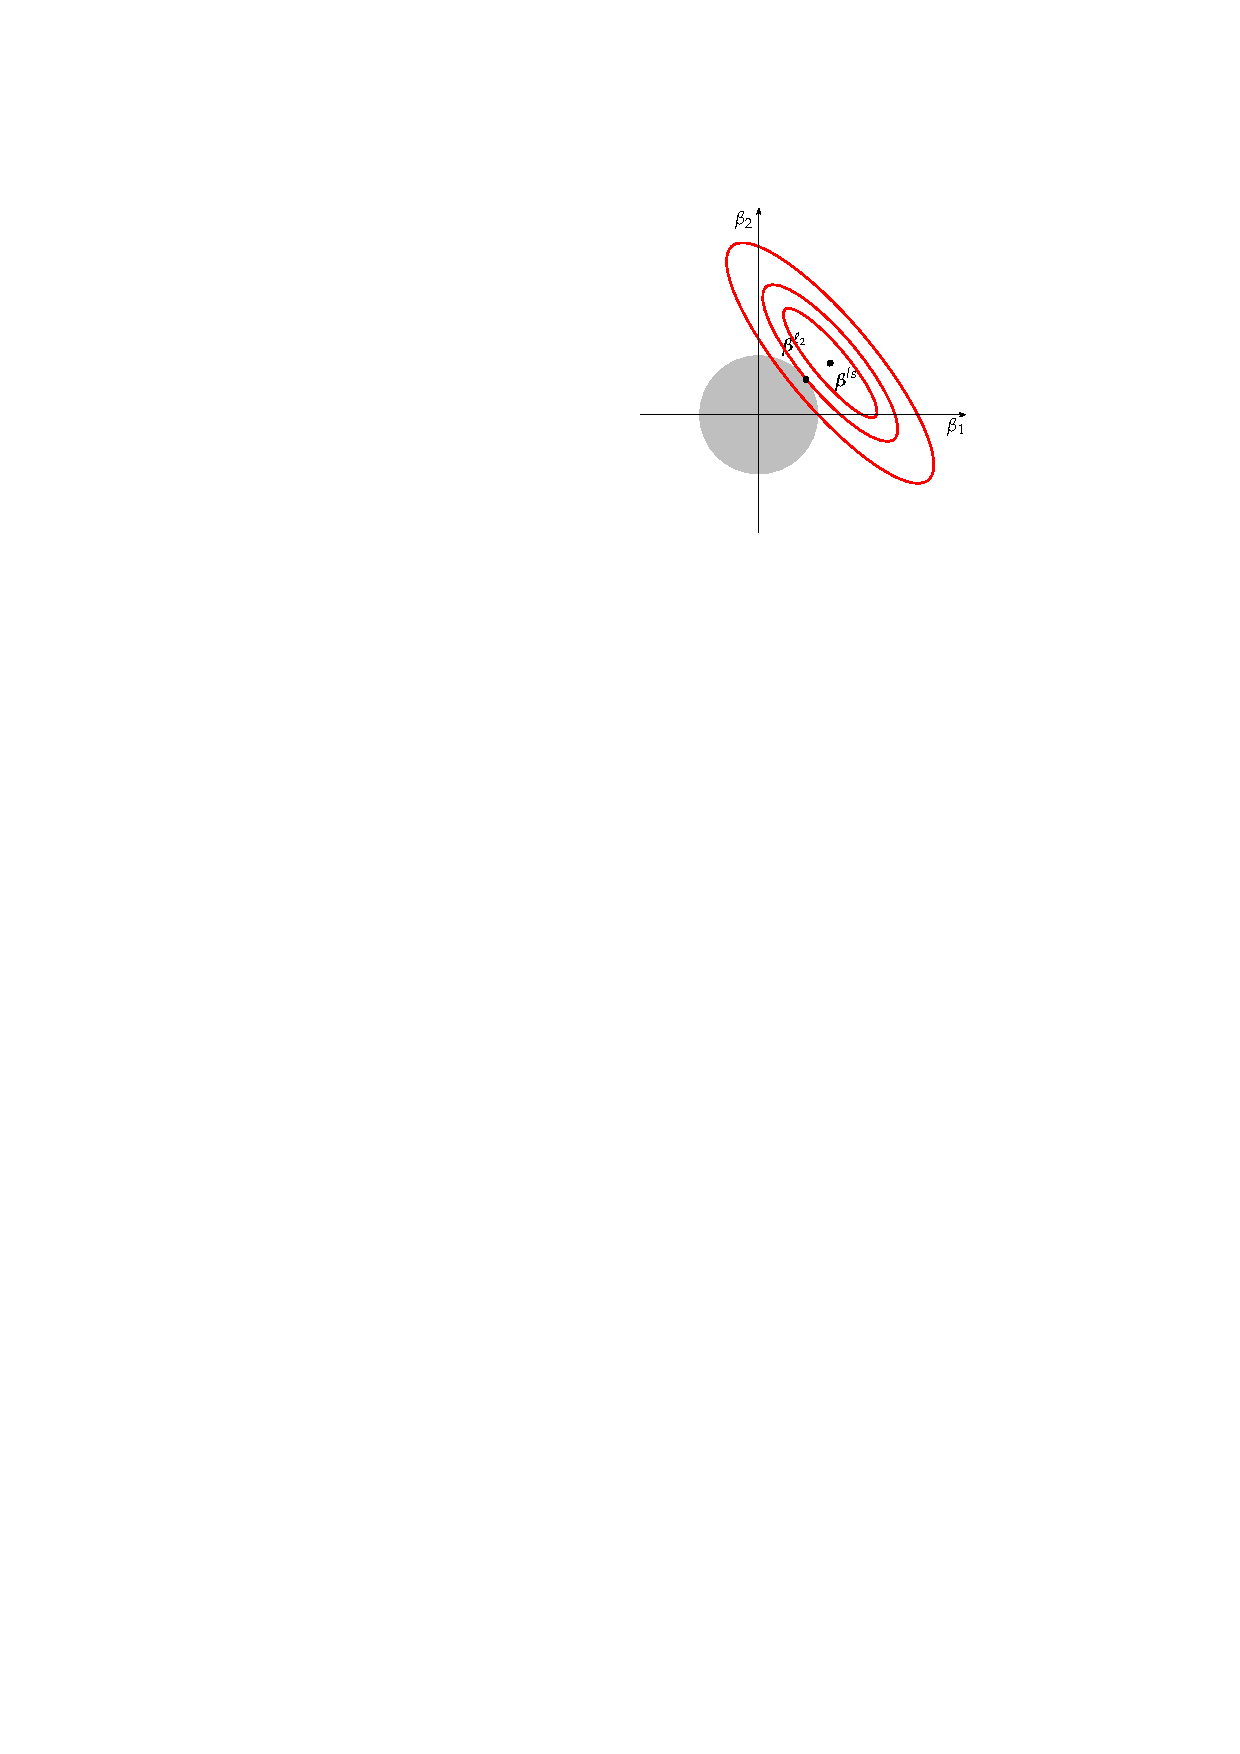
\includegraphics[width=.7\textwidth]{figures/ridge_set}
      \end{column}
    \end{columns}
  \end{overlayarea}
\end{frame}

\begin{frame}
  \frametitle{A 2-dimensional toy example}

  Consider that the true relationship is $Y = X_1 \beta_1 + X_2\beta_2
  +  \varepsilon$ If  $X_1$ and  $X_2$ are  strongly  correlated, then
  $X_1\approx X_2$ and for any $\gamma\geq 0$
  \begin{align*}
    Y & = X_1 (\beta_1 + \gamma) + X_2 (\beta_2 - \gamma) +
    \gamma(X_1-X_2) + \varepsilon \\
    & \approx X_1 (\beta_1 + \gamma) + X_2 (\beta_2 - \gamma) + \varepsilon.
  \end{align*}
  A large  panel of fit  with estimated $\bbeta$ varying  according to
  $\gamma$ will produce the same prediction error.

  \vfill

  \onslide<2>{
    For small $s$ (or large $\lambda$ in the Lagrangian form), the ridge
    controls
    \begin{equation*}
      (\beta_1 + \gamma)^2 + (\beta_2 - \gamma)^2
    \end{equation*}
    which  is minimal for  $\gamma =  (\beta_2-\beta_1)/2$, and  in this
    case $\beta_j = (\beta_1 + \beta_2)/2$.
  }
\end{frame}







\begin{frame}[containsverbatim,allowframebreaks]
  \frametitle{A 2-dimensional toy example (in \texttt{R})}

Generate two correlated predictors
\begin{knitrout}\scriptsize
\definecolor{shadecolor}{rgb}{0.969, 0.969, 0.969}\color{fgcolor}\begin{kframe}
\begin{alltt}
\hlkwd{suppressMessages}\hlstd{(}\hlkwd{library}\hlstd{(quadrupen))} \hlcom{# use github version}
\hlstd{x1} \hlkwb{<-} \hlkwd{rnorm}\hlstd{(}\hlnum{5}\hlstd{)}
\hlstd{x2} \hlkwb{<-} \hlstd{x1} \hlopt{+} \hlkwd{rnorm}\hlstd{(}\hlnum{5}\hlstd{,}\hlnum{0}\hlstd{,} \hlnum{0.5}\hlstd{)}
\hlkwd{cor}\hlstd{(x1,x2)}
\end{alltt}
\begin{verbatim}
## [1] 0.7316593
\end{verbatim}
\end{kframe}
\end{knitrout}

Draw $Y$ and plot the  \alert{\bf ridge regularisation path}
\begin{knitrout}\scriptsize
\definecolor{shadecolor}{rgb}{0.969, 0.969, 0.969}\color{fgcolor}\begin{kframe}
\begin{alltt}
\hlkwd{library}\hlstd{(glmnet)}
\hlstd{y} \hlkwb{<-} \hlstd{x1} \hlopt{+} \hlstd{x2} \hlopt{+}\hlkwd{rnorm}\hlstd{(}\hlnum{5}\hlstd{)}
\hlkwd{plot}\hlstd{(quadrupen}\hlopt{::}\hlkwd{ridge}\hlstd{(}\hlkwd{cbind}\hlstd{(x1,x2),y))}
\end{alltt}


{\ttfamily\noindent\bfseries\color{errorcolor}{\#\# Error: 'ridge' is not an exported object from 'namespace:quadrupen'}}\end{kframe}
\end{knitrout}

\end{frame}

\begin{frame}
  \frametitle{Ridge as penalized regression}

  \alert{Dont  penalize   the  intercept}  thus  consider   $\bbeta  =
  (\beta_1,\dots\beta_p)$ and set
  \begin{itemize}
  \item $\hatbeta_0 = \bar{\by} - \bar{x}\hatbbeta$
  \item center $\mathbf{y}$ and $\mathbf{x}_j$, $j=1,\dots,p$.
  \end{itemize}
  \alert{Standardize the $\bx_j$} for the fit and send back
  $\hatbbetaridge$ to the \alert{orginal scale}.

  \vfill

  \begin{block}{Convex Langrangian form}
    \vspace{-.5cm}
    \begin{align*}
      \hat{\bbeta}^{\text{ridge}} &  =   \argmin_{\bbeta\in\R^p}  \frac{1}{2}
      \|\mathbf{y} - \mathbf{X} \bbeta\|^2 + \lambda \|\bbeta\|^2\\
      & = (\mathbf{X}^\intercal \mathbf{X} +
      \lambda \mathbf{I}_p)^{-1} \mathbf{X}^\intercal \mathbf{y} = \mathbf{H}_\lambda \by.
    \end{align*}
  \end{block}

  \vfill

  \begin{block}{Strong convexity}
    Oppositely to  the least squares, a  non-singular solution always
    exists   when    $\lambda>0$   whatever   the    conditioning   of
    $\mathbf{X}^\intercal \mathbf{X}$ (original proposal).
  \end{block}

\end{frame}

% \subsubsection{Propriétés et résolution pratique}

% \begin{frame}
%   \frametitle{Connexion à l'OLS}

%   Soit $\mathbf{S}_\lambda =  \mathbf{X}^\intercal \mathbf{X} + \lambda
%   \mathbf{I}_p$.  Alors
%   \begin{equation*}
%     \hat{\bbeta}^{\text{ridge}} =
%     \mathbf{S}_\lambda^{-1}        \mathbf{X}^\intercal       \mathbf{X}
%     \hat{\bbeta}^{\text{ols}} =
%     \left(\mathbf{I}_p - \lambda\mathbf{S}_\lambda^{-1}\right) \hat{\bbeta}^{\text{ols}}.
%   \end{equation*}
%   Lorsque       $\lambda=0$,       $\hat{\bbeta}^{\text{ridge}}$      et
%   $\hat{\bbeta}^{\text{ols}}$ coincident.

%   \begin{columns}
%     \begin{column}[c]{.5\textwidth}
%       Dans le cas d'un design orthonormal, $\mathbf{X}^\intercal
%       \mathbf{X}=\mathbf{I}$ et
%       \begin{equation*}
%         \hat{\bbeta}^{\text{ridge}} = \frac{1}{1+\lambda} \hat{\bbeta}^{\text{ols}}.
%       \end{equation*}
%     \end{column}

%     \begin{column}[c]{.5\textwidth}
%       \begin{center}
%         \begin{tikzpicture}[scale=.5,font=\small]
%           \draw[very thin,color=gray] (-4,-4) grid [xstep=1,ystep=1] (4,4);
%           \draw[->] (-4.5,0) -- (4.5,0) node[right] {$\beta^{\text{ols}}$};
%           \draw[->] (0,-4.5) -- (0,4.5) ;
%           \draw[color=blue] plot[samples=200] (\x,{1/(2)*\x})
%           node[right] {Ridge};
%           \draw[dashed,color=black] plot (\x,{\x}) node[right] {OLS};

%           % units for cartesian reference frame
%           \foreach \x in {-4,-2,0,2,4}{
%             \draw (\x cm,1pt)  -- (\x cm,-3pt)
%             node[anchor=north,xshift=-0.09cm] {\scriptsize$\x$};
%             \draw (1pt,\x cm) -- (-3pt,\x cm)
%             node[anchor=east] {\scriptsize$\x$};
%           }
%         \end{tikzpicture}
%       \end{center}
%     \end{column}
%   \end{columns}

% \end{frame}

% \begin{frame}
%   \frametitle{Biais et variance de l'estimateur Ridge}

%   \begin{proposition}
%     \begin{equation*}
%       \E\left(\hat{\bbeta}^{\text{ridge}}-\hatbbetaols\right)   =
%       -\lambda \mathbf{S}_\lambda^{-1} \bbeta,       \var\left(\hat{\bbeta}^{\text{ridge}}\right)  =
%       \sigma^2 \mathbf{S}_\lambda^{-1} \mathbf{X}^\intercal \mathbf{X}
%       \mathbf{S}_\lambda^{-1}.
%     \end{equation*}
%     et
%     \begin{equation*}
%       \var(\hatbbetaols) - \var(\hatbbetaridge) \succeq 0
%     \end{equation*}
%     donc
%     $\var(x^T\hatbbetaols) \geq \var(x^T\hatbbetaridge)$ un $x$ fixé.
%   \end{proposition}

%   \vfill

%   \begin{itemize}
%   \item quand $\lambda\to 0$, sans biais, grande variance (OLS)
%   \item quand $\lambda\to \infty$, grand biais, variance nulle.
%   \end{itemize}

%   \vfill

%   $\rightsquigarrow$  Un compromis  est nécessaire  (\textit{i.e.}, un bon choix pour $\lambda$).

% \end{frame}

% \begin{frame}
%   \frametitle{Calcul pratique du chemin de solution}
%   \framesubtitle{Ridge et SVD}

%   \begin{block}{Décomposition en valeur singulière --
%       \href{{http://upload.wikimedia.org/wikipedia/commons/e/e9/Singular_value_decomposition.gif}}{lien
%         vers une illustration}}
%     \begin{equation*}
%       \mathbf{X} = \mathbf{U} \mathbf{D} \mathbf{V}^\intercal,
%     \end{equation*}
%     \vspace{-.5cm}
%     \begin{itemize}
%     \item  $\mathbf{U}$  est  une   matrice  $n\times  p$  orthogonale
%       génératrice de l'espace colonne,
%     \item  $\mathbf{V}$  est  une   matrice  $p\times  p$  orthogonale
%       génératice de l'espace ligne,
%     \item     $\mathbf{D}=     \mathrm{diag}(d_1,\dots,d_i,\dots,d_p)$
%       contient les valeurs singulières de $\mathbf{X}$.
%     \end{itemize}
%   \end{block}

%   \vfill

%   \begin{equation*}
%     \hat{\bbeta}^{\mathrm{ridge}}      =      \mathbf{V}
%     {\boldsymbol\Delta}_\lambda \mathbf{U}^\intercal \mathbf{y},
%   \end{equation*}
%   où ${\boldsymbol\Delta}_\lambda$ est une matrice diagonale telle que
%   $\Delta_i= d_i/(d_i^2+\lambda)$.

%   \vfill

%   \begin{block}{Coût algorithmique}
%     Le calcul du chemin de solution complet pour $K$ valeurs de $\lambda$ nécessite
%     \begin{enumerate}
%     \item une SVD ($\mathcal{O}(np^2)$)
%     \item un produit matriciel entre $\mathbf{V}$ et la matrice $p\times K$
%           ${\boldsymbol\Delta}_\lambda     \mathbf{U}^\intercal
%       \mathbf{y}$
%     \end{enumerate}
%   \end{block}
% \end{frame}







\begin{frame}[containsverbatim]
  \frametitle{Ridge fit for the prostate cancer data}

  \vfill

Compute the ridge path
\begin{knitrout}\scriptsize
\definecolor{shadecolor}{rgb}{0.969, 0.969, 0.969}\color{fgcolor}\begin{kframe}
\begin{alltt}
\hlstd{ridge_path} \hlkwb{<-} \hlstd{quadrupen}\hlopt{::}\hlkwd{ridge}\hlstd{(x_train, y_train)}
\end{alltt}


{\ttfamily\noindent\bfseries\color{errorcolor}{\#\# Error: 'ridge' is not an exported object from 'namespace:quadrupen'}}\end{kframe}
\end{knitrout}

\vfill

Compute the prediction error on the test set for all $\lambda$
\begin{knitrout}\scriptsize
\definecolor{shadecolor}{rgb}{0.969, 0.969, 0.969}\color{fgcolor}\begin{kframe}
\begin{alltt}
\hlstd{err} \hlkwb{<-} \hlkwd{colMeans}\hlstd{((y_test} \hlopt{-} \hlkwd{predict}\hlstd{(ridge_path,} \hlkwd{as.matrix}\hlstd{(x_test)))}\hlopt{^}\hlnum{2}\hlstd{)}
\end{alltt}


{\ttfamily\noindent\bfseries\color{errorcolor}{\#\# Error in predict(ridge\_path, as.matrix(x\_test)): object 'ridge\_path' not found}}\end{kframe}
\end{knitrout}

\vfill

Then, $\lambda^\star$ that minimizes this error
\begin{knitrout}\scriptsize
\definecolor{shadecolor}{rgb}{0.969, 0.969, 0.969}\color{fgcolor}\begin{kframe}
\begin{alltt}
\hlstd{ridge_path}\hlopt{@}\hlkwc{lambda2}\hlstd{[}\hlkwd{which.min}\hlstd{(err)]}
\end{alltt}


{\ttfamily\noindent\bfseries\color{errorcolor}{\#\# Error in eval(expr, envir, enclos): object 'ridge\_path' not found}}\end{kframe}
\end{knitrout}

The prediction error is smaller than with the OLS
\begin{knitrout}\scriptsize
\definecolor{shadecolor}{rgb}{0.969, 0.969, 0.969}\color{fgcolor}\begin{kframe}
\begin{alltt}
\hlstd{err_ridge} \hlkwb{<-} \hlstd{err[}\hlkwd{which.min}\hlstd{(err)]}
\end{alltt}


{\ttfamily\noindent\bfseries\color{errorcolor}{\#\# Error in eval(expr, envir, enclos): object 'err' not found}}\begin{alltt}
\hlkwd{print}\hlstd{(err_ridge)}
\end{alltt}


{\ttfamily\noindent\bfseries\color{errorcolor}{\#\# Error in print(err\_ridge): object 'err\_ridge' not found}}\begin{alltt}
\hlkwd{print}\hlstd{(err_ols)}
\end{alltt}
\begin{verbatim}
## [1] 0.0673631
\end{verbatim}
\end{kframe}
\end{knitrout}

\end{frame}

\begin{frame}[containsverbatim]
\begin{knitrout}\scriptsize
\definecolor{shadecolor}{rgb}{0.969, 0.969, 0.969}\color{fgcolor}\begin{kframe}


{\ttfamily\noindent\bfseries\color{errorcolor}{\#\# Error in plot(ridge\_path): object 'ridge\_path' not found}}\end{kframe}
\end{knitrout}
\end{frame}


\subsubsection{Model complexity and Tuning parameter}

\begin{frame}
   \frametitle{Classical options}

 \begin{block}{Cross-validation}
   We compute $CV(\lambda)$, the CV error along the $\lambda$ path
    \begin{enumerate}
    \item if $K=n$, this is the LOOCV,
    \item if $K=2$, this is the hold out estimation,
    \item in a high dimensional setup, we must choose $K$ ``carefully'',
    \end{enumerate}
   We choose  $\lambda$ minimising the CV 
  \end{block}

\vfill

\begin{block}{Penalized criteria}
We choose  $\lambda$ minimizing a criterion with the form
\begin{equation*}
\mathrm{crit}(\lambda) = \mathrm{err}_\mathcal{D}(\lambda) + \mathrm{pen}(\mathrm{df}_\lambda)
\end{equation*}
$\rightsquigarrow$ What sens give to the degrees of freedom for ridge regression?
\end {block}

\end{frame}


\begin{frame}
  \frametitle{Effective degrees of freedom}

  \begin{itemize}
  \item Degrees of freedom of a model describes its complexity level.
  \item For the least squares, $\mathrm{df} = p$ (plus 1 for the intercept).
  \item Need a definition adapted to shrinkage methods.
  \end{itemize}

  \vfill

  \begin{definition}[Efron  and  others]   Consider  a  fitted  vector
    $\hat{\mathbf{y}}$ from an observation $\mathbf{y}$. We define its
    degrees of freedom as
    \begin{equation*}
      \mathrm{df}(\hat{\mathbf{y}})    =    \frac{1}{\sigma^2}
      \sum_{i=1}^n \mathrm{cov}(\hat{y}_i,y_i).
    \end{equation*}
    $\rightsquigarrow$The  harder the fit  to the  data, the  higher the
    covariance.
  \end{definition}

\end{frame}

\begin{frame}
  \frametitle{Effective degrees of freedom: the ridge case}

  \begin{proposition} Consider a linear fitting method that predicts
    $\hat{\mathbf{y}}$  for  entry  $\mathbf{y}$  through  the
    smoother matrix $\mathbf{H}$:
    \begin{equation*}
      \hat{\mathbf{y}} = \mathbf{H} \mathbf{y}.
    \end{equation*}
    The    effective    degrees    of    freedom    of    the    model
    $\hat{\mathbf{y}}$ verifies
    \begin{equation*}
      \mathrm{df}(\hat{\mathbf{y}}) = \mathrm{Tr}(\mathbf{H}).
    \end{equation*}
  \end{proposition}

  \vfill

  \begin{block}{Ridge: effective degrees of freedom}
    For ridge  regression, $\mathrm{df}$  is a decreassig  function of
    $\lambda$ which tends to 0 (or 1 when considering the intercept):
    \begin{equation*}
      \mathrm{df}(\hat{\mathbf{y}}_\lambda) =\sum_{i=1}^p \frac{d_i^2}{d_i^2+\lambda}.
    \end{equation*}
  \end{block}


\end{frame}
 




\begin{frame}[containsverbatim]
  \frametitle{Cross-Validation}
  
  Cross-validation is easily parallelized and is fast on small data sets

\begin{knitrout}\scriptsize
\definecolor{shadecolor}{rgb}{0.969, 0.969, 0.969}\color{fgcolor}\begin{kframe}
\begin{alltt}
\hlkwd{system.time}\hlstd{(loo} \hlkwb{<-} \hlstd{quadrupen}\hlopt{::}\hlkwd{crossval}\hlstd{(x_train,y_train,} \hlkwc{penalty} \hlstd{=}  \hlstr{"ridge"}\hlstd{,} \hlkwc{K} \hlstd{= n))}
\end{alltt}


{\ttfamily\noindent\bfseries\color{errorcolor}{\#\# Error in match.arg(penalty): 'arg' should be one of "{}elastic.net"{}, "{}bounded.reg"{}}}\end{kframe}
\end{knitrout}

\begin{knitrout}\scriptsize
\definecolor{shadecolor}{rgb}{0.969, 0.969, 0.969}\color{fgcolor}\begin{kframe}
\begin{alltt}
\hlkwd{system.time}\hlstd{(CV10} \hlkwb{<-} \hlstd{quadrupen}\hlopt{::}\hlkwd{crossval}\hlstd{(x_train,y_train,} \hlkwc{penalty} \hlstd{=}  \hlstr{"ridge"}\hlstd{,} \hlkwc{K} \hlstd{=} \hlnum{10}\hlstd{))}
\end{alltt}


{\ttfamily\noindent\bfseries\color{errorcolor}{\#\# Error in match.arg(penalty): 'arg' should be one of "{}elastic.net"{}, "{}bounded.reg"{}}}\end{kframe}
\end{knitrout}

\end{frame}

\begin{frame}[containsverbatim]
  \frametitle{Leave one out}
\begin{knitrout}\scriptsize
\definecolor{shadecolor}{rgb}{0.969, 0.969, 0.969}\color{fgcolor}\begin{kframe}


{\ttfamily\noindent\bfseries\color{errorcolor}{\#\# Error in plot(loo, main = "{}LOO CV error"{}): object 'loo' not found}}\end{kframe}
\end{knitrout}
\end{frame}

\begin{frame}[containsverbatim]
  \frametitle{Ten fold}
\begin{knitrout}\scriptsize
\definecolor{shadecolor}{rgb}{0.969, 0.969, 0.969}\color{fgcolor}\begin{kframe}


{\ttfamily\noindent\bfseries\color{errorcolor}{\#\# Error in plot(CV10, main = "{}10-fold CV error"{}): object 'CV10' not found}}\end{kframe}
\end{knitrout}
\end{frame}





\subsection{Lasso Regression}

\subsubsection{Definition of the LASSO estimator}

\begin{frame}
  \frametitle{The Lasso}
  \framesubtitle{Least Absolute Shrinkage and Selection Operator}

  \begin{block}{Fact}
    Ridge  performs  regularization\dots but  we  also  would like  to
    select the most significant variables.
  \end{block}

  \vfill

  \begin{block}{Idea}
    Suggest  an admissible  set that  induces  \alert{sparsity} (force
    several entries to exactly zero in $\hat{\bbeta}$).
  \end{block}

  \vfill

  \begin{overlayarea}{\textwidth}{.4\textheight}
    \begin{columns}
      \begin{column}[c]{.6\textwidth}
        \begin{block}{Lasso as a convex optimization problem}
          The Lasso estimate $\hat{\bbeta}^{\text{lasso}}$ solves
          \begin{equation*}
            \minimize_{\bbeta\in\R^{p+1}} \mathrm{RSS}(\bbeta), \quad \text{s.t.  }  \sum_{j=1}^p
            \left|\beta_j\right|  \leq s,
          \end{equation*}
          where $s$ is a shrinkage factor.
        \end{block}
      \end{column}
      \begin{column}{.4\textwidth}
        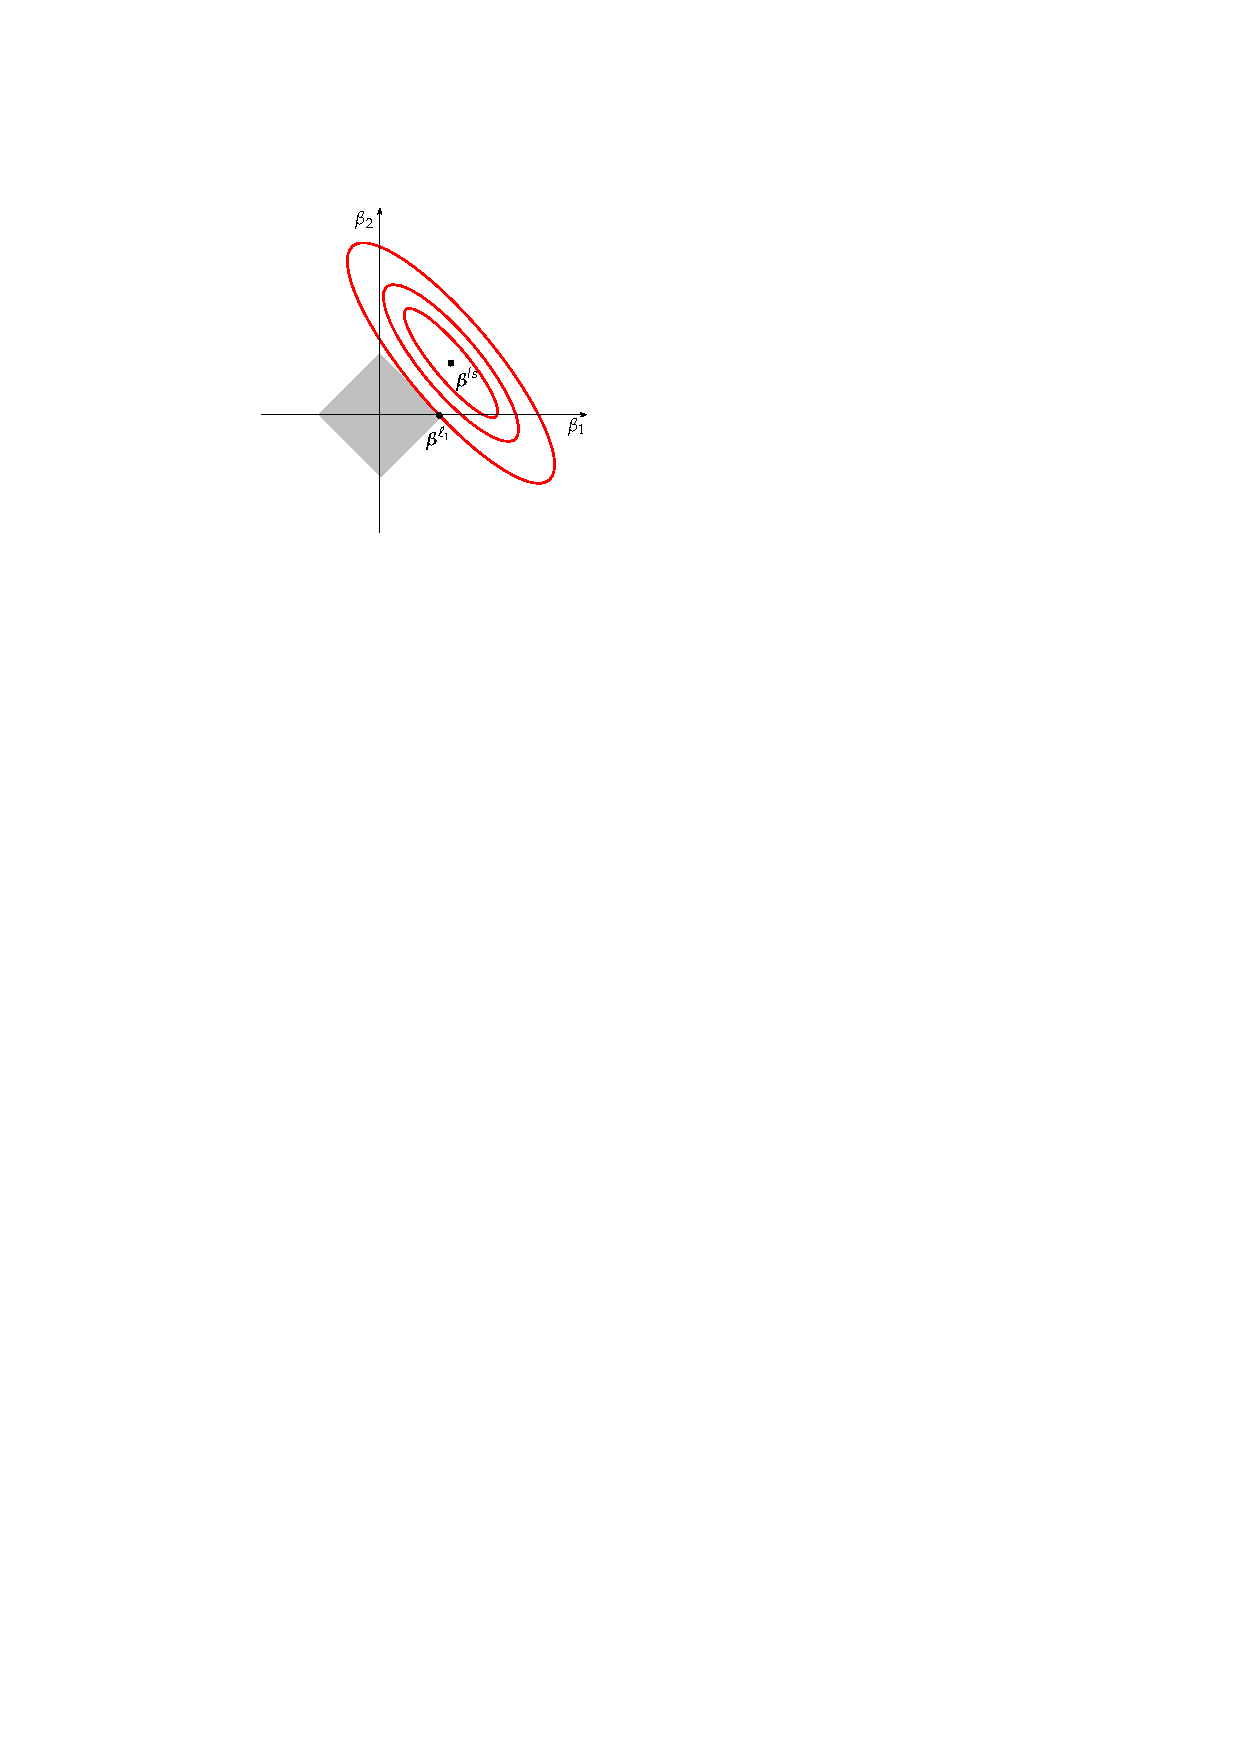
\includegraphics[width=.7\textwidth]{figures/lasso_set}
      \end{column}
    \end{columns}
  \end{overlayarea}

\end{frame}

\begin{frame}
  \frametitle{Some more insights: 2-dimensional example}
  \framesubtitle{Thanks to Sylvie Huet}

  \begin{overlayarea}{\textwidth}{\textheight}

    \begin{equation*}
      \sum_{i=1}^n (y_i-x_i^1\beta_1 - x_i^2\beta_2)^2, \qquad
      \only<1>{\text{no constraints}}
      \only<2>{\text{s.c. } |\beta_1| + |\beta_2| < 0.75}
      \only<3>{\text{s.c. } |\beta_1| + |\beta_2| < 0.66}
      \only<4>{\text{s.c. } |\beta_1| + |\beta_2| < 0.4}
      \only<5>{\text{s.c. } |\beta_1| + |\beta_2| < 0.2}
      \only<6>{\text{s.c. } |\beta_1| + |\beta_2| < 0.0743}
    \end{equation*}

    \includegraphics<1>[width=.7\textwidth]{dess11}
    \includegraphics<2>[width=.7\textwidth]{dess12}
    \includegraphics<3>[width=.7\textwidth]{dess13}
    \includegraphics<4>[width=.7\textwidth]{dess14}
    \includegraphics<5>[width=.7\textwidth]{dess15}
    \includegraphics<6>[width=.7\textwidth]{dess16}

  \end{overlayarea}

\end{frame}

\begin{frame}
  \frametitle{Lasso as penalized regression}

  \begin{block}{Get rid of  the intercept}
    We should not penalize the intercept term, thus
    \begin{itemize}
    \item $\hat{\beta}_0 = \bar{\mathbf{y}}$,
    \item center $\mathbf{y}$ and $\mathbf{x}_j$, $j=1,\dots,p$,
    \item scale the predictor before the fit,
    \item send $\hatbbeta$ back to the original scale.
    \end{itemize}
  \end{block}

  \vfill

 Solve the convex, $\ell_1$-penalized problem
  \begin{equation*}
      \hat{\bbeta}^{\text{lasso}}   =   \argmin_{\bbeta\in\R^p}  \frac{1}{2}
      \|\mathbf{y} - \mathbf{X} \bbeta\|^2 + \lambda \|\bbeta\|_1,
  \end{equation*}
  whose solution has no close form, but always exists and is unique as
  soon as $\mathbf{X}^\intercal \mathbf{X}$ has full rank.

  \vfill

  $\rightsquigarrow$  Lasso   performs  regularization   and  variable
  selection but has no analytical solution.

\end{frame}





\begin{frame}[containsverbatim,allowframebreaks]
  \frametitle{Lasso fit on the prostate cancer data}

  \vfill
Compute the LASSO path
\begin{knitrout}\scriptsize
\definecolor{shadecolor}{rgb}{0.969, 0.969, 0.969}\color{fgcolor}\begin{kframe}
\begin{alltt}
\hlkwd{library}\hlstd{(glmnet)}
\hlstd{lasso_path} \hlkwb{<-} \hlstd{quadrupen}\hlopt{::}\hlkwd{lasso}\hlstd{(x_train,y_train)}
\end{alltt}


{\ttfamily\noindent\bfseries\color{errorcolor}{\#\# Error: 'lasso' is not an exported object from 'namespace:quadrupen'}}\end{kframe}
\end{knitrout}

\vfill

Compute the prediction error on the test set for all $\lambda$

\begin{knitrout}\scriptsize
\definecolor{shadecolor}{rgb}{0.969, 0.969, 0.969}\color{fgcolor}\begin{kframe}
\begin{alltt}
\hlstd{err} \hlkwb{<-} \hlkwd{colMeans}\hlstd{((y_test} \hlopt{-} \hlkwd{predict}\hlstd{(lasso_path, x_test))}\hlopt{^}\hlnum{2}\hlstd{)}
\end{alltt}


{\ttfamily\noindent\bfseries\color{errorcolor}{\#\# Error in predict(lasso\_path, x\_test): object 'lasso\_path' not found}}\end{kframe}
\end{knitrout}

\vfill

Then, $\lambda^\star$ that minimizes this error
\begin{knitrout}\scriptsize
\definecolor{shadecolor}{rgb}{0.969, 0.969, 0.969}\color{fgcolor}\begin{kframe}
\begin{alltt}
\hlstd{lasso_path}\hlopt{@}\hlkwc{lambda1}\hlstd{[}\hlkwd{which.min}\hlstd{(err)]}
\end{alltt}


{\ttfamily\noindent\bfseries\color{errorcolor}{\#\# Error in eval(expr, envir, enclos): object 'lasso\_path' not found}}\end{kframe}
\end{knitrout}

\framebreak

The prediction error is smaller than with the OLS with only 5 coefficients
\begin{knitrout}\scriptsize
\definecolor{shadecolor}{rgb}{0.969, 0.969, 0.969}\color{fgcolor}\begin{kframe}
\begin{alltt}
\hlstd{err[}\hlkwd{which.min}\hlstd{(err)]}
\end{alltt}


{\ttfamily\noindent\bfseries\color{errorcolor}{\#\# Error in eval(expr, envir, enclos): object 'err' not found}}\begin{alltt}
\hlstd{lasso_path}\hlopt{@}\hlkwc{coefficients}\hlstd{[}\hlkwd{which.min}\hlstd{(err), ]}
\end{alltt}


{\ttfamily\noindent\bfseries\color{errorcolor}{\#\# Error in eval(expr, envir, enclos): object 'lasso\_path' not found}}\end{kframe}
\end{knitrout}

\end{frame}

\begin{frame}[containsverbatim]
  \frametitle{Prediction error on the test set}

\begin{knitrout}\scriptsize
\definecolor{shadecolor}{rgb}{0.969, 0.969, 0.969}\color{fgcolor}\begin{kframe}
\begin{alltt}
\hlkwd{qplot}\hlstd{(}\hlkwd{log10}\hlstd{(lasso_path}\hlopt{@}\hlkwc{lambda1}\hlstd{), err)} \hlopt{+} \hlkwd{geom_line}\hlstd{()} \hlopt{+}
\hlkwd{geom_vline}\hlstd{(}\hlkwc{xintercept} \hlstd{=} \hlkwd{log10}\hlstd{(lasso_path}\hlopt{@}\hlkwc{lambda1}\hlstd{[}\hlkwd{which.min}\hlstd{(err)]),} \hlkwc{lty}\hlstd{=}\hlnum{3}\hlstd{)}
\end{alltt}


{\ttfamily\noindent\bfseries\color{errorcolor}{\#\# Error in data.frame(xintercept = xintercept): object 'lasso\_path' not found}}\end{kframe}
\end{knitrout}
\end{frame}

\begin{frame}[containsverbatim]
  \frametitle{Path of solution ($\lambda$)}

\begin{knitrout}\scriptsize
\definecolor{shadecolor}{rgb}{0.969, 0.969, 0.969}\color{fgcolor}\begin{kframe}
\begin{alltt}
\hlkwd{plot}\hlstd{(lasso_path)}
\end{alltt}


{\ttfamily\noindent\bfseries\color{errorcolor}{\#\# Error in plot(lasso\_path): object 'lasso\_path' not found}}\end{kframe}
\end{knitrout}
\end{frame}


\begin{frame}[containsverbatim]
  \frametitle{Path of solution (amount of shrinkage $s$)}

\begin{knitrout}\scriptsize
\definecolor{shadecolor}{rgb}{0.969, 0.969, 0.969}\color{fgcolor}\begin{kframe}
\begin{alltt}
\hlkwd{plot}\hlstd{(lasso_path,} \hlkwc{xvar}\hlstd{=}\hlstr{"fraction"}\hlstd{)}
\end{alltt}


{\ttfamily\noindent\bfseries\color{errorcolor}{\#\# Error in plot(lasso\_path, xvar = "{}fraction"{}): object 'lasso\_path' not found}}\end{kframe}
\end{knitrout}
\end{frame}

\subsubsection{Model complexity and Tuning parameter}

\begin{frame}
  \frametitle{Critères pénalisés}

  \begin{block}{LASSO degrees of freedom}
    It simply equals the number of active (non-null) coefficients)
\[
\mathrm{df}(\hat{\by}_\lambda^{\text{lasso}}) = \mathrm{card}(\set{j:\beta_j(\lambda)\neq 0}) = |\mathcal{A}|.
\]
  \end{block}

  \begin{itemize}
    \item \alert{Akaike Information Criterion} 
        \begin{equation*}
          \mathrm{AIC} = -2 \mathrm{loglik} + 2\frac{|\mathcal{A}|}{n},
        \end{equation*}
      \item \alert{Bayesian   Information   Criterion}
        \begin{equation*}
          \mathrm{BIC} = -2\mathrm{loglik} + |\mathcal{A}|\log(n),
        \end{equation*}
      \item \alert{modified BIC} (when $n < p$)
        \begin{equation*}
          \mathrm{mBIC} = -2\mathrm{loglik} + |\mathcal{A}|\log(p),
        \end{equation*}
      \item \alert{Extended BIC} add a prior on the number of model with size  $|\mathcal{A}|$
        \begin{equation*}
          \mathrm{eBIC} = -2\mathrm{loglik} + |\mathcal{A}|(\log(n) + 2\log(p)).
        \end{equation*}
      \end{itemize}
\end{frame}





\begin{frame}[containsverbatim]
 \frametitle{Cancer de la prostate}
 \framesubtitle{Calcul de l' AIC/BIC en estimant $\sigma$ (plot)}

\begin{knitrout}\scriptsize
\definecolor{shadecolor}{rgb}{0.969, 0.969, 0.969}\color{fgcolor}\begin{kframe}


{\ttfamily\noindent\bfseries\color{errorcolor}{\#\# Error in criteria(lasso\_path): could not find function "{}criteria"{}}}\end{kframe}
\end{knitrout}
\end{frame}

\begin{frame}[containsverbatim]
  \frametitle{Cross-validation}

\begin{knitrout}\scriptsize
\definecolor{shadecolor}{rgb}{0.969, 0.969, 0.969}\color{fgcolor}\begin{kframe}
\begin{alltt}
\hlkwd{system.time}\hlstd{(loo} \hlkwb{<-} \hlkwd{crossval}\hlstd{(x_train, y_train,} \hlkwc{penalty} \hlstd{=} \hlstr{"lasso"}\hlstd{,} \hlkwc{K} \hlstd{= n))}
\end{alltt}


{\ttfamily\noindent\bfseries\color{errorcolor}{\#\# Error in match.arg(penalty): 'arg' should be one of "{}elastic.net"{}, "{}bounded.reg"{}}}\end{kframe}
\end{knitrout}

\begin{knitrout}\scriptsize
\definecolor{shadecolor}{rgb}{0.969, 0.969, 0.969}\color{fgcolor}\begin{kframe}
\begin{alltt}
\hlkwd{system.time}\hlstd{(CV10} \hlkwb{<-} \hlkwd{crossval}\hlstd{(x_train, y_train,} \hlkwc{penalty} \hlstd{=} \hlstr{"lasso"}\hlstd{,} \hlkwc{K} \hlstd{=} \hlnum{10}\hlstd{))}
\end{alltt}


{\ttfamily\noindent\bfseries\color{errorcolor}{\#\# Error in match.arg(penalty): 'arg' should be one of "{}elastic.net"{}, "{}bounded.reg"{}}}\end{kframe}
\end{knitrout}

\end{frame}

\begin{frame}[containsverbatim]
  \frametitle{Leave one out}
\begin{knitrout}\scriptsize
\definecolor{shadecolor}{rgb}{0.969, 0.969, 0.969}\color{fgcolor}\begin{kframe}


{\ttfamily\noindent\bfseries\color{errorcolor}{\#\# Error in plot(loo, main = "{}LOO CV error"{}): object 'loo' not found}}\end{kframe}
\end{knitrout}
\end{frame}



\begin{frame}[containsverbatim]
  \frametitle{Ten fold}
\begin{knitrout}\scriptsize
\definecolor{shadecolor}{rgb}{0.969, 0.969, 0.969}\color{fgcolor}\begin{kframe}


{\ttfamily\noindent\bfseries\color{errorcolor}{\#\# Error in plot(CV10, main = "{}10-fold CV error"{}): object 'CV10' not found}}\end{kframe}
\end{knitrout}
\end{frame}





\end{document}

